% ============================================================
% ICLR 2027 — restructured on the form-vs-content spine (21-ago).
% Single source of truth: every number traces to a CSV named in a % comment.
% Figures included use ONLY clean regenerated data (fig_excess_panel,
% fig_text_nulls, fig_bestmetric_scatter) or data-independent originals
% (fig_tree_visualization, fig3_causal). The stale-data
% originals (fig_scaling, fig_synthesis_pooled, gain bubbles) are NOT
% referenced and must be regenerated before any future use.
% ============================================================
\documentclass{article}
\usepackage{iclr2027_conference,times}

\usepackage[utf8]{inputenc}
\usepackage[T1]{fontenc}
\usepackage{hyperref}
\usepackage{url}
\usepackage{booktabs}
\usepackage{array}
\usepackage{amsthm}
\usepackage{amsfonts}
\usepackage{amsmath}
\usepackage{nicefrac}
\usepackage{microtype}
\usepackage{xcolor}
\usepackage{graphicx}
\usepackage{subcaption}
\usepackage{multirow}
\usepackage{enumitem}
\usepackage{placeins}
\usepackage{float}
\usepackage{overpic}

% Title chosen by Javi (21-ago). Alternatives kept for coauthor veto:
%  (b) The Platonic Tree Is Ours: Whose Hierarchy Foundation Models Grow
%  (c) Whose Tree Does a Foundation Model Grow? Revisiting the PRH in Geometry
% Earlier candidates ("Grow Their Own Trees", "Form, not Content") were
% partially invalidated by the tree-map result: supervised/contrastive models
% share essentially one tree.
\title{Is There a Platonic Tree? \\ Calibrating Latent Hyperbolicity \\ in Foundation Models}

\author{Anonymous authors}

%\iclrfinalcopy % Uncomment for camera-ready version, but NOT for submission.

\newtheoremstyle{inline}{3pt}{3pt}{}{}{\bfseries}{.}{ }{}
\newtheoremstyle{inlineit}{3pt}{3pt}{\itshape}{}{\bfseries}{.}{ }{}
\theoremstyle{inline}
\newtheorem{definition}{Definition}
\theoremstyle{inlineit}
\newtheorem{proposition}{Proposition}
\makeatletter\g@addto@macro\normalsize{\setlength\abovedisplayskip{3pt plus 1pt}\setlength\belowdisplayskip{3pt plus 1pt}\setlength\abovedisplayshortskip{2pt}\setlength\belowdisplayshortskip{2pt}}
% typographic only (page budget, 2026-09-18; tightened 2026-09-21 for priorities 1b and 2): the section headings and the run-in paragraph headings open with less white space than the style's default; fonts, margins and line spacing are the style's
\renewcommand\section{\@startsection{section}{1}{\z@}{-0.3ex plus -0.3ex minus -.2ex}{0.2ex plus 0.2ex minus 0.1ex}{\large\sc\raggedright}}
\renewcommand\subsection{\@startsection{subsection}{2}{\z@}{-0.3ex plus -0.3ex minus -.2ex}{0.2ex plus .2ex}{\normalsize\sc\raggedright}}
\renewcommand\paragraph{\@startsection{paragraph}{4}{\z@}{0ex plus 0.3ex minus .2ex}{-1em}{\normalsize\bf}}\makeatother
\setlength{\textfloatsep}{4pt plus 2pt minus 2pt}\setlength{\abovecaptionskip}{0pt}\setlength{\parskip}{0pt plus 1pt}
% rebuttal version = the frozen submission file plus the parallel-track paragraphs (phaseE_rebuttal.py); the frozen text and numbers are unchanged
% final version: classic structure, plain prose (author's brief of 2026-09-18); generated by rebuttal/scripts/phaseE_submission.py.
\begin{document}

\maketitle
\raggedbottom   % final pass: [t] figures and [H] tables leave short pages; ragged bottoms instead of underfull vertical boxes

\begin{abstract}
Hyperbolic representation learning rests on a premise we call latent hyperbolicity: standard models are already tree-like because their class geometry scores a low Gromov $\delta$, a measure of tree-likeness that is zero for a tree. That low value is also what a random cloud of the same dimension and spread scores, so we build an instrument that reads every score as its excess over many such clouds, and a hierarchy test whose ability to detect a hierarchy is measured. We apply it to 12 vision backbones, 6 datasets and 15 text models. On image features, where the premise is read, the calibrated reading is indistinguishable from a random cloud in most model--dataset cells and small elsewhere. Class centroids do carry structure that a random cloud of the same shape does not, in 44 of 72 cells, but so does a star of clusters. In 4 of 12 ImageNet backbones the hierarchy test finds structure, but it is the orientation of clusters relative to the superclass centers, not a hierarchy among those centers: randomizing orientations removes it, whereas a planted hierarchy, synthetic or trained in, survives. Where a planted hierarchy is detected, in 9 of 12 backbones, no hierarchy as strong as the planted one is found; in the other 3 the test cannot tell. MERU, trained in hyperbolic space, shows the same structure as its Euclidean twin in a space that stays nearly flat. In text, the result depends on the model's recipe and size. Across models, the trees agree on which classes group together well above chance, though less than two readings of the same model, and not on distances; the self-supervised models organize classes by direction rather than by distance, which a comparison by distance misses. Read correctly, foundation models organize classes into clusters that they partly share, show no hierarchy among the superclasses where the test can see one, and their raw tree-likeness is not evidence for hyperbolic geometry.
\end{abstract}

\section{Introduction}
\label{sec:introduction}

Semantic knowledge is hierarchical, and hyperbolic space is the natural geometric home for hierarchies \citep{nickel2017poincare, sarkar2011low, ganea2018hyperbolic, chami2019hyperbolic}. A line of work therefore imposes it on representations at training time, from vision to vision--language and language \citep{Khrulkov_2020_CVPR, ermolov2022hyperbolic, atigh2022hyperbolic, bdeir2024fully, desai2023meru, pal2025compositional, chen2022fully, he2026helm, sinha2024learning}. These methods cite a premise, which we call \emph{latent hyperbolicity}: standard models already organize concepts in a tree-like metric structure. The evidence is a single number, the Gromov $\delta$ of their features, which is zero for a metric tree and grows as a metric departs from one. Measured on CNN and ViT features \citep{Khrulkov_2020_CVPR, bdeir2024fully}, on token embeddings \citep{yang2025hyperbolic} and on word vectors \citep{tifrea2019poincare}, it comes out low. Those readings are taken at the sample level, on individual images or tokens rather than on classes, and they are read against the ideal values of a tree and of a non-hyperbolic space, never against what a structureless cloud of the same dimension and spectrum would score. Is the premise right, and what does it license? Figure~\ref{fig:concept} frames the question: an observer who sees only a shadow, the raw $\delta$, asks which of three worlds cast it, a structureless cloud, a star of clusters or a tree. All three read alike.

\begin{figure}[t]
\centering
\IfFileExists{figures/fig1_concept.pdf}%
{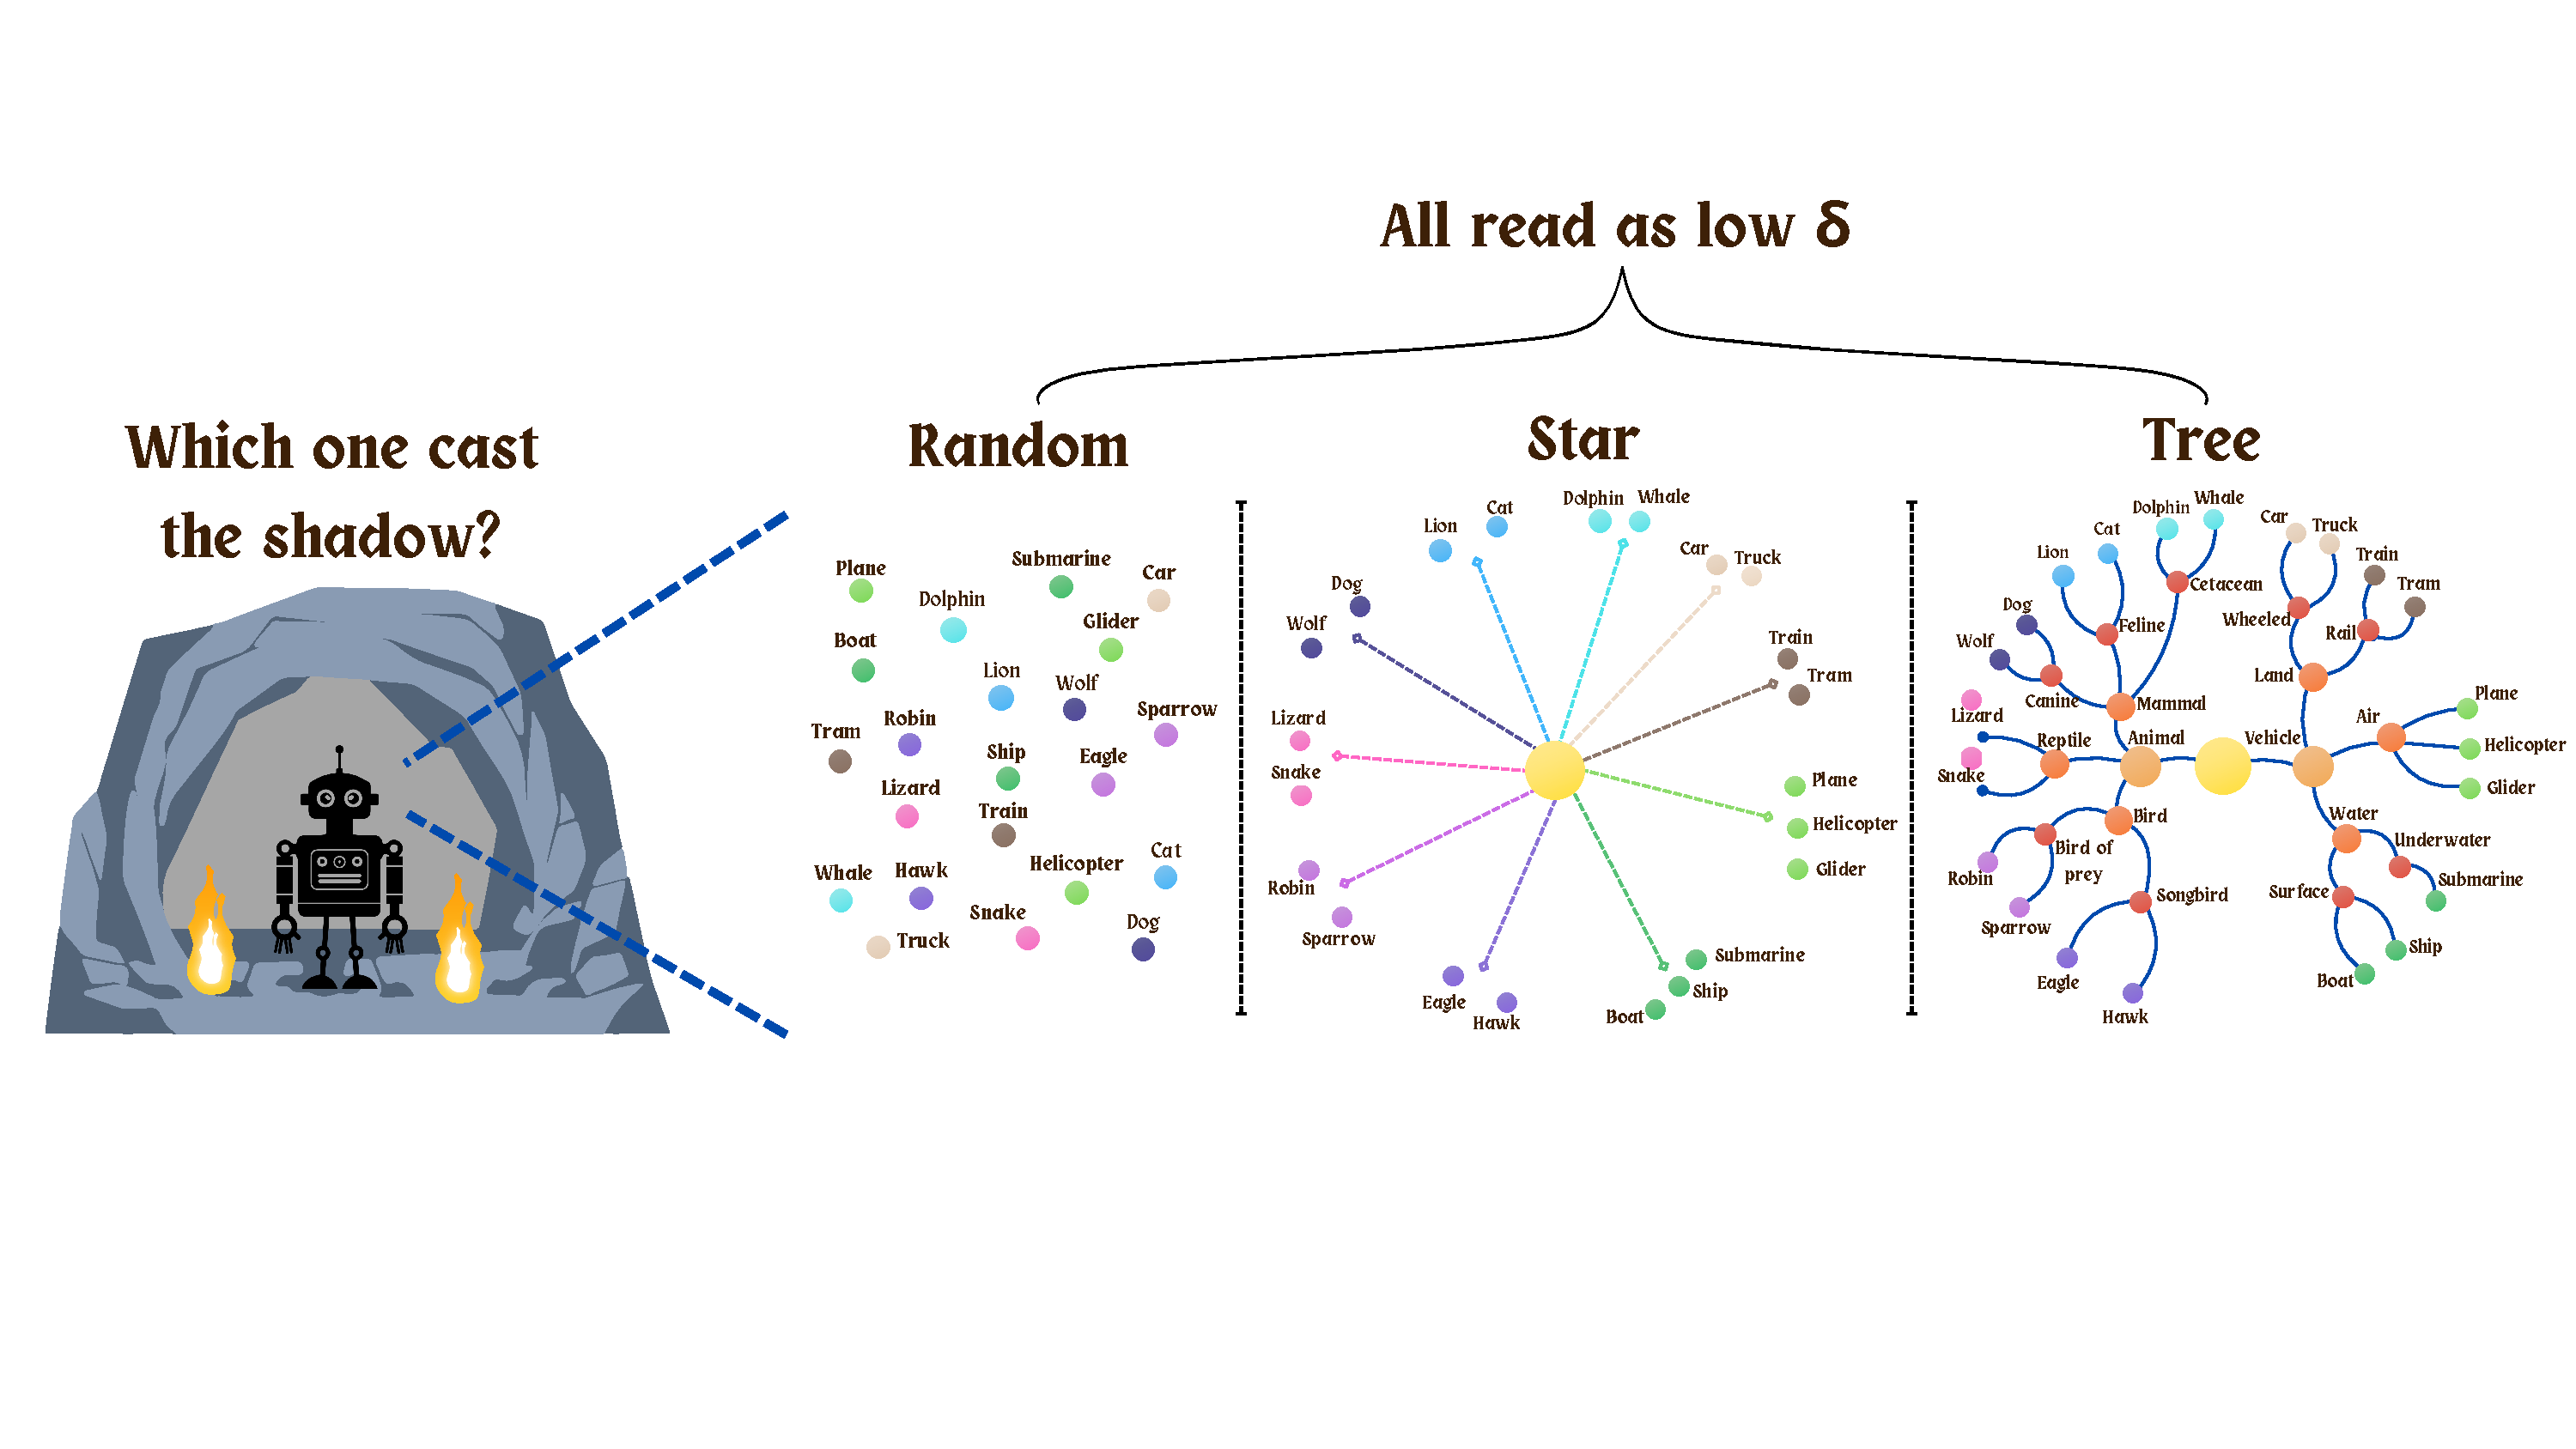
\includegraphics[width=\textwidth, trim=23 229 3 232]{figures/fig1_concept.pdf}}
{\fbox{\parbox[c][1.4in][c]{\dimexpr\textwidth-2\fboxsep-2\fboxrule\relax}{\centering \texttt{figures/fig1\_concept.pdf} (conceptual figure, drawn by the authors; same-size placeholder)}}}
\vspace{2pt}
\caption{\textbf{Plato's cave: a random cloud, a star and a tree cast the same shadow.} An observer who sees only shadows cannot tell which object cast them, and a raw $\delta$ is such a shadow: points with no structure, clusters around a hub, and a nested hierarchy all read as low $\delta$. The instrument reads the objects instead of the shadow: the excess separates the random cloud from the other two, and the hierarchy test separates the star from the tree.}
\label{fig:concept}
\end{figure}

Why is the reading low? Gromov $\delta$ assigns zero to trees \citep{Gromov1987}, but its reference level depends on dimension, spectrum and statistic, so a raw value cannot be called low on its own. High-dimensional clouds concentrate toward equidistance \citep{beyer1999nearest, aggarwal2001surprising}, which is a degenerate star tree: we call this the \emph{dimension confound}, the geometric counterpart of the width confounder of \citet{groger2026aristotelian}. Anisotropic spectra lower the effective dimension and raise the reading: the \emph{spectrum confound}. And the supremum over sampled quadruples grows with the budget and does not converge \citep{fournier2015computing}: the \emph{statistic confound}.

We build the instrument that reads $\delta$ against the right reference. It calibrates the estimator on reference geometries, expresses every reading as an \emph{excess} over a null cloud matched in dimension and covariance spectrum, ranks that excess against matched replicates, and adds a \emph{hierarchy test} whose false-alarm rate and power are measured on real clouds. With it we ask of geometry what convergence work asks of similarity \citep{huh2024platonic, groger2026aristotelian}: what survives calibration, and is it shared? \citet{groger2026aristotelian} calibrate similarity across models; we calibrate geometry within a model, and comparing trees across models needs a calibration of its own.

\textbf{The answer has three parts.} (i) \emph{Where the premise is read,} on image features, the calibrated reading is indistinguishable from a random cloud of the same shape in most model--dataset cells and small elsewhere. The 4 values reported by \citet{Khrulkov_2020_CVPR} are reproduced and, calibrated, 2 of them are indistinguishable from a random cloud, 3 under their own statistic. (ii) \emph{Within each model,} class centroids carry structure that a random cloud does not have, in 44 of 72 cells and 30 of 36 on datasets with 47 classes or more, but a star of clusters already produces it. The hierarchy test finds more in 4 of 12 ImageNet backbones: the orientation of each cluster relative to its superclass center, which we call its hub, not a hierarchy among the hubs. Randomizing the orientations removes every verdict, whereas an implanted hierarchy, synthetic or trained in, survives. In the 9 of 12 backbones where an implanted hierarchy is detected, none as strong is found; in the other 3 the test is blind. A backbone trained in hyperbolic space shows the same structure as its Euclidean twin and stays nearly flat. (iii) \emph{Across models,} the trees agree on which classes group together well above chance, though less than two readings of the same model, and not on distances; the self-supervised models organize classes by direction rather than by distance, which a comparison by distance misses.

\textbf{Our contributions are:}
\begin{enumerate}[topsep=0pt,itemsep=1pt,leftmargin=*]
\item \textbf{The instrument.} A calibrated reading of $\delta$, compared with random clouds of the same shape, and a hierarchy test whose false-alarm rate and power are measured on real clouds.
\item \textbf{The census.} The premise calibrated where it is read, including a published reading reproduced; structure beyond a random cloud in most models; clusters oriented toward their hubs in a few; no hierarchy among the hubs where the test can see one; and a hyperbolic-trained backbone as the control for imposing the geometry.
\item \textbf{The map of trees.} Across models, the trees agree on which classes group together but not on distances, and the self-supervised models organize classes by direction, which a comparison by distance misses.
\item \textbf{Consequences for practice.} The rule that derives curvature from a raw $\delta$ assigns curvature to random clouds; we say what to measure before imposing curvature, and cosine collects most of the structure at no cost.
\end{enumerate}

\section{Related Work}
\label{sec:related}

Reading $\delta$ against a matched reference has precedent in network science, where the $\delta$ of real graphs is compared with that of random graphs of comparable size \citep{narayan2011curvature, kennedy2013hyperbolicity, adcock2013treelike}. We bring the idea to embedding clouds, where the reference must match dimension and spectrum. The curvature itself has been studied as a representation tradeoff \citep{sala2018representation} and as a mixed-curvature product to be learned \citep{gu2019learning}, which presupposes a diagnostic of the kind we calibrate. The analyses of learned representations characterize Euclidean structure and do not test for tree-likeness: representation similarity, intrinsic dimension and neural collapse \citep{kornblith2019cka, ansuini2019intrinsic, pope2021intrinsic, papyan2020prevalence}. Closest to us is the work on representational convergence: the Platonic Representation Hypothesis \citep{huh2024platonic} argues that models converge toward shared representations, and its cross-modal convergence has been stress-tested at scale \citep{koepke2026cave}; \citet{groger2026aristotelian} show that permutation-calibrated similarity removes most of that convergence while local neighborhood structure survives, and \citet{park2024geometry} read concept hierarchy in language models from the orthogonality of concept directions. We are the geometric complement of this program: the same calibration applied within a model instead of across models. It adds a hierarchy test measured on real clouds, a hyperbolic backbone as the control for imposing the geometry, and a calibration of the tree-to-tree comparison itself.

\section{Methodology}
\label{sec:instrument}

\subsection{Background: Gromov $\delta$}
\label{sec:f-gromov}

Tree-likeness is measured on quadruples. Take any four points $w,x,y,z$ of a metric space with distance $d$. They can be paired in three ways, and each pairing has a sum of two distances:
\begin{equation}
d(w,x)+d(y,z),\qquad d(w,y)+d(x,z),\qquad d(w,z)+d(x,y).
\label{eq:pairings}
\end{equation}
Sort the three sums as $S_{\max}\ge S_{\mathrm{mid}}\ge S_{\min}$. In a tree the two largest sums are always equal, because the two pairings that cross the trunk traverse the same path, so the four-point defect $(S_{\max}-S_{\mathrm{mid}})/2$ is zero. The further a metric is from a tree, the larger the defect can become. A metric tree has $\delta=0$. Euclidean space has no bound at all: enlarging a square enlarges its defect in proportion. Hyperbolic space sits in between, with a bounded defect whose value for the hyperbolic plane is known, $\ln 2$ under this definition \citep{nica2016strong}.

\begin{definition}[four-point defect]
\label{def:defect}
For a quadruple $(w,x,y,z)$ with the pairing sums of Eq.~\ref{eq:pairings} sorted as $S_{\max}\ge S_{\mathrm{mid}}\ge S_{\min}$, the four-point defect is $\delta(w,x,y,z)=\tfrac12\,(S_{\max}-S_{\mathrm{mid}})$, and the Gromov $\delta$ of a metric space is the supremum of the defect over its quadruples \citep{Gromov1987}.
\end{definition}

\subsection{Estimation and normalization}
\label{sec:f-estimation}

Three steps turn $\delta$ into a number that can be compared across models. First, a thousand centroids have far more quadruples than can be enumerated, so the defect is computed on half a million random quadruples. Second, the largest defect in that sample is a poor estimate of the supremum: it belongs to a single extreme quadruple and keeps growing as more quadruples are drawn \citep{fournier2015computing}. We therefore read the 99.9th percentile of the sampled defects, $\hat\delta_{99.9}$, the value that 99.9 per cent of them fall below. It keeps the tail of the defects, as the supremum does, but it is set by hundreds of quadruples rather than by one. It also does not move with the sample size: across quadruple budgets the ImageNet reading drifts by less than half its own spread (Table~\ref{tab:q8-robust}). Third, the defect grows with the size of the point set, so we divide by the diameter, the largest pairwise distance:
\begin{equation}
\delta_{\text{norm}}=\frac{\hat\delta_{99.9}}{\mathrm{diam}}.
\label{eq:deltanorm}
\end{equation}
On this scale a tree reads zero, and a hyperbolic region of radius four or more reads below a sphere (Table~\ref{tab:q10-calibration}).

\begin{definition}[reading of record]
\label{def:record}
The reading of record of a cloud is $\delta_{\text{norm}}$ of Eq.~\ref{eq:deltanorm}, with $\hat\delta_{99.9}$ computed over half a million sampled quadruples per seed and averaged over 10 seeds.
\end{definition}

\begin{proposition}[range bound and dimension confound]
\label{prop:bound}
Let $d_{\min}$ and $d_{\max}$ be the smallest and the largest pairwise distance of a finite metric space. (a) For any quadruple the four-point defect is at most $d_{\max}-d_{\min}$, hence $\delta_{\text{norm}}\le 1-d_{\min}/d_{\max}$. (b) For an iid Gaussian cloud of $n$ points in dimension $d$, with $n$ fixed, $d_{\min}/d_{\max}\to1$ as $d$ grows \citep{beyer1999nearest, aggarwal2001surprising}, so $\delta_{\text{norm}}\to0$ without any structure.
\end{proposition}

\paragraph{A raw value cannot be called low on its own.} Proposition~\ref{prop:bound} makes the dimension confound precise; the calibration on reference geometries shows the spectrum and statistic confounds (Table~\ref{tab:q10-calibration}).

\subsection{Spectrum-matched null, excess and genuineness}
\label{sec:f-null}

\begin{definition}[Haar null]
\label{def:null}
A null replicate is a cloud with the real shape and no structure. Let $X=U\Sigma V^{\top}$ be the singular value decomposition of the centered cloud; the replicate is $X'=Q\Sigma V^{\top}$ with $Q$ the orthogonal factor of a column-centered Gaussian matrix, orthogonal to the all-ones vector and Haar-distributed on the centered subspace, so $X'$ has exactly the centered singular values of $X$ and structureless coefficients.
\end{definition}

\paragraph{The null is a cloud with the real shape and no structure.} Of the two constructions compared, Gaussian coefficients reproduce the spectrum only on average and inflate the excess of low-rank clouds. The centered Haar construction reproduces the centered spectrum exactly, so it is the record. The uncentered and the Gaussian readings are reported beside it (Table~\ref{tab:q1-census}).

\begin{definition}[excess]
\label{def:excess}
With $K$ null replicates $X'_1,\dots,X'_K$ of Definition~\ref{def:null}, the excess of a cell is
\begin{equation}
e(X)=\delta_{\text{norm}}(X)-\frac{1}{K}\sum_{k=1}^{K}\delta_{\text{norm}}(X'_k).
\label{eq:excess}
\end{equation}
\end{definition}

\paragraph{Size and evidence.} The excess is a size; the evidence is the rank of the reading among its replicates and the left-tail $p$ that the rank gives,
\begin{equation}
r=\#\{k:\ \delta_{\text{norm}}(X'_k)>\delta_{\text{norm}}(X)\},\qquad p=\frac{1+K-r}{K+1},\qquad K=200.
\label{eq:rank}
\end{equation}

\begin{definition}[genuine]
\label{def:genuine}
Order the $m$ left-tail $p$-values of a census as $p_{(1)}\le\dots\le p_{(m)}$. A model--dataset cell is genuine when its $p$ is at or below the Benjamini--Hochberg threshold at level five per cent,
\begin{equation}
p\ \le\ p_{(i^{*})},\qquad i^{*}=\max\{i:\ p_{(i)}\le 0.05\, i/m\},
\label{eq:bh}
\end{equation}
and the word is used in this sense only.
\end{definition}

\paragraph{What a genuine excess means.} A negative genuine excess, more than chance would give, certifies structure beyond the second moments; clustering is its most plausible reading, supported by the superclass recovery of Section~\ref{sec:content}. Two cells of the same dataset can have the same reading and opposite verdicts (Figure~\ref{fig:overview}).

\begin{figure}[t]
\centering

\includegraphics[width=\linewidth]{figures/fig_overview_final.pdf}
\caption{\textbf{The raw reading cannot be read on its own.} (a) Raw reading and matched null per ImageNet backbone, ordered by dimension; the gap is the excess. (b) Same dataset, same reading, opposite verdict: ViT-B on CIFAR-100 images and DINO-B on CIFAR-100 centroids. % exp1_delta_controls.csv, expR52_census_haar_p999_200.csv, expR62_samplelevel_record.csv, final_fig2b.json
}
\label{fig:overview}
\end{figure}

\subsection{Hierarchy test}
\label{sec:f-depthtest}

\paragraph{Why a second test.} A genuine excess can come from clusters alone, so a second test asks whether the clusters are themselves arranged hierarchically. It needs three constructions.

\begin{definition}[hub null and excess B]
\label{def:hubnull}
Given a grouping of classes into superclasses, which we call the frame, assigning each centroid $x_i$ to a cluster $k(i)$ with hub $h_{k(i)}$, the cluster mean, write $x_i=h_{k(i)}+o_i$. The hub null keeps every offset $o_i$ and replaces the hubs by a Haar resample with their spectrum, $x'_i=h'_{k(i)}+o_i$, and the excess of Eq.~\ref{eq:excess} against this null, $e_B$, measures structure above the clusters of the frame only.
\end{definition}

\begin{definition}[matched star]
\label{def:star}
The matched star of a cloud keeps the real clusters, each as a Haar sample with the cluster's own covariance, and places their hubs as Gaussian draws at the real hub radius: the clustering of the real cloud with no hierarchy above it. Its spectrum-matched-hub variant draws the hubs as a Haar resample of the real hubs.
\end{definition}

\begin{definition}[decoupling control]
\label{def:decoupling}
The decoupling control keeps the hubs of the frame and rotates each cluster's offsets by an independent Haar rotation. A verdict that survives the decoupling is carried by the arrangement of the hubs; one that does not is carried by the orientation of the clusters relative to their hubs, which we call alignment.
\end{definition}

\paragraph{The hierarchy test compares the real cloud with its matched star.} With $e_B$ read on the real cloud and on its matched star, the depth statistic and its standardized form are
\begin{equation}
\mathrm{depth}=e_B(X)-e_B(X_{\mathrm{star}}),\qquad z=\mathrm{depth}\,/\,\mathrm{s.d.},
\label{eq:depth}
\end{equation}
The spread is taken over star seeds and null replicates, and a cloud is certified against its matched star when $z\le-2$. The power of the test is the fraction of implanted hierarchies it detects, and its false-alarm rate is the fraction of flat controls that fire. Both are measured on real clouds in Section~\ref{sec:f-depth}.

\subsection{Comparing trees across models}
\label{sec:f-treemap}

\paragraph{Trees are compared under a configuration chosen before the comparison.} Two hierarchies are compared by the adjusted Rand index between their cut partitions and by the correlation of their cophenetic distances. They are also compared by their agreement on which pair of a random class triplet merges first. The configuration of metric and linkage is selected per dataset by a criterion fixed without reference to the agreements. It is the highest cophenetic fidelity among configurations whose reference cuts are non-degenerate for every model. Local agreement is read with the permutation calibration of \citet{groger2026aristotelian} on mutual-kNN agreement and centroid CKA.

\subsection{Projection and tasks}
\label{sec:f-projection}

\paragraph{Three readouts are compared on the intact representation.} A parameter-free map centers the features, scales the 95th-percentile norm to radius $1/\sqrt2$ and preserves directions. Euclidean, cosine and Poincar\'{e} readouts are then scored by nearest-centroid classification and 5-way 5-shot episodes on every cell of the task grid. % exp1, exp2

\section{Experimental Setup}
\label{sec:f-setup}

\paragraph{The census has 12 backbones, 6 class sets and 15 text models.} The vision backbones are 4 supervised ViTs trained on ImageNet-21k, DINO-B, 4 DINOv2 sizes, CLIP-B, CLIP-L and SigLIP-B. The class sets are ImageNet and CIFAR-100, which carry a real hierarchy, CIFAR-10 and DTD, and the flat FMNIST and MNIST. The text models read the thousand ImageNet class names: 4 GPT-2 sizes, 3 Pythia sizes, OLMo-1B and 7 sentence embedders (Table~\ref{tab:q14-panel}).

\paragraph{Four controls test the alternatives.} Two self-supervised ResNets read the vision census. DeiT-B and the augreg ViT-B, trained on ImageNet-1k leaf labels, test whether a hierarchical label set explains the alignment. MERU and its Euclidean CLIP twin test whether training in hyperbolic space creates depth. The census ViT-B, fine-tuned with and without a hierarchical objective, is the trained control.

\paragraph{The premise is read on images and hierarchy on centroids.} The sample-level reading uses about a thousand stratified training images per cell on CIFAR-100 and DTD. Class centroids average a hundred cached training images per class on ImageNet and the full cached split elsewhere. Causal language models give the last-token state of ``a photo of a \{class\}'', extracted one prompt at a time because batching alters GPT-2's hidden states. Embedders use their recommended pooling (Table~\ref{tab:q2-text}).

\paragraph{Calibration budget and frames.} Each cell is read against 200 Haar replicates, with half a million sampled quadruples per seed and 10 seeds. With 10 classes there are only 210 quadruples, so $\hat\delta_{99.9}$ coincides with the supremum there. Benjamini--Hochberg runs over the vision census and, separately, over the text census. The frame, the grouping into superclasses, is the WordNet cut into 30 superclasses on ImageNet and the 20 coarse labels on CIFAR-100. A balanced grouping is the control, with 10 star seeds.

\section{Results}
\label{sec:form}

\subsection{The premise at the sample level}
\label{sec:f-sample}

\paragraph{The premise does not survive calibration where it is read.} On per-image features, where the premise is read, the calibrated reading is not genuine in most cells, that is, no more than chance would give. Where it is genuine, the excess removes at most two fifths of the null reading. Table~\ref{tab:q3-sample} gives the reading per cell. % expR62_samplelevel_record.csv

\paragraph{A published reading is reproduced and calibrated.} Their estimator was run on our extraction; it reproduces the raw $\delta_{\text{rel}}$ that \citet{Khrulkov_2020_CVPR} report for ResNet-34 on 4 datasets within 0.03. Calibrated, CIFAR-10 and CUB-200 are indistinguishable from a random cloud, and CIFAR-100 and MiniImageNet fall below it. Under their own statistic, the supremum, calibrated against the same replicates, CIFAR-100 joins CIFAR-10 and CUB-200 among the indistinguishable, and only MiniImageNet falls below the random cloud. Table~\ref{tab:khrulkov} gives the 4 rows. % expR78_khrulkov_replication_summary.csv, expR85_khrulkov_sup_summary.csv

% prov: expR78_khrulkov_replication_summary.csv
\begin{table}[t]
\centering
\footnotesize
\setlength{\tabcolsep}{5pt}
\begin{tabular}{lcccc}
\toprule
dataset & their $\delta_{\text{rel}}$ & ours, their estimator & excess & $r$/200, largest $p$ \\
\midrule
CIFAR-10 & 0.26 & 0.275 & $-0.0037$ & 173/200, 0.333 \\
CIFAR-100 & 0.25 & 0.261 & $-0.0087$ & 198/200, 0.030 \\
CUB-200 & 0.25 & 0.270 & $-0.0043$ & 177/200, 0.249 \\
MiniImageNet & 0.21 & 0.203 & $-0.0234$ & 200/200, 0.005 \\
\bottomrule
\end{tabular}
\caption{\textbf{A published reading reproduced and calibrated.} ResNet-34 setting of \citet{Khrulkov_2020_CVPR}: their relative hyperbolicity, ours with their estimator, the excess over the matched null, and the rank of 200 replicates with the largest left-tail $p$ over batches. % expR78_khrulkov_replication_summary.csv
}
\label{tab:khrulkov}
\end{table}


\subsection{Structure beyond the second moments at the class level}
\label{sec:f-class}

\begin{figure}[t]
\centering

\includegraphics[width=\linewidth]{figures/fig_excess_final.pdf}
\caption{\textbf{Most cells show structure beyond the second moments.} Excess of the reading of record over its matched null per dataset and backbone, filled when genuine; band: two null standard deviations. % expR52_census_haar_p999_200.csv
}
\label{fig:excess}
\end{figure}

\begin{table}[t]
\centering
\small
\setlength{\tabcolsep}{3.4pt}
\begin{tabular}{l l c c c c c c}
\toprule
model & family & $\hat\delta_{99.9}$ IN & excess IN & $r$/200 ($p$) & exc.\ C100 & exc.\ C10 & $\rho_{\text{WN}}$ \\
\midrule
ViT-T & sup. & $0.088$ & $-0.005^{\circ}$ & 169 (.159) & $-0.006^{\circ}$ & $-0.012^{\circ}$ & $+0.52$ \\
ViT-S & sup. & $0.063$ & $-0.012$ & 200 (.005) & $-0.000^{\circ}$ & $-0.042$ & $+0.50$ \\
ViT-B & sup. & $0.054$ & $-0.016$ & 200 (.005) & \textbf{$+0.006^{\circ}$} & $-0.038$ & $+0.49$ \\
ViT-L & sup. & $0.055$ & $-0.016$ & 200 (.005) & $-0.020$ & $-0.037$ & $+0.53$ \\
\midrule
DINO-B & SSL & $0.055$ & $-0.020$ & 200 (.005) & $-0.031$ & $-0.042$ & $+0.36$ \\
DINOv2-S & SSL & $0.053$ & $-0.016$ & 200 (.005) & $-0.030$ & $-0.033$ & $+0.22$ \\
DINOv2-B & SSL & $0.034$ & $-0.017$ & 200 (.005) & $-0.031$ & $-0.065$ & $+0.18$ \\
DINOv2-L & SSL & $0.030$ & $-0.014$ & 200 (.005) & $-0.034$ & $-0.084$ & $+0.18$ \\
DINOv2-G & SSL & $0.033$ & $-0.008$ & 200 (.005) & $-0.039$ & $-0.077$ & $+0.20$ \\
\midrule
CLIP-B & contr. & $0.084$ & $-0.007^{\circ}$ & 172 (.144) & $-0.019$ & $-0.022^{\circ}$ & $+0.57$ \\
CLIP-L & contr. & $0.076$ & $-0.009$ & 197 (.020) & $-0.018$ & $-0.020^{\circ}$ & $+0.59$ \\
SigLIP-B & contr. & $0.075$ & $-0.008^{\circ}$ & 189 (.060) & $-0.022$ & $-0.027$ & $+0.58$ \\
\bottomrule
\end{tabular}
\caption{\textbf{Clustered structure is the rule at the class level.} Per backbone: raw ImageNet reading $\hat\delta_{99.9}$, excess over the Haar null mean, rank $r$/200 with left-tail $p$, genuine = BH $p\le0.05$ over 72 cells ($^{\circ}$: not genuine; bold: above the null), the CIFAR-100 and CIFAR-10 excess, and $\rho_{\text{WN}}$, the Spearman correlation with WordNet distances. % expR75_census_centered_haar.csv, exp3_alignment.csv
}
\label{tab:census}
\end{table}


\paragraph{Most cells show structure beyond the second moments.} It is genuine in 44 of 72 cells and 30 of 36 on the 3 datasets with 47 classes or more. On ImageNet and CIFAR-100 the count is 18 of 24. Figure~\ref{fig:excess} and Table~\ref{tab:census} give the census. % expR52_census_haar_p999_200.csv

\paragraph{The count survives resampling.} Folding image resampling and the estimator's seeds into the null spread, or repeating the census on resampled centroids, keeps most of the count. Table~\ref{tab:q8-robust} gives the bootstrap. % expR66_joint_sensitivity_summary.csv

\paragraph{The structure depends on the class set more than on the model.} The smallest backbone is genuine on one dataset only, and the flat datasets have smaller and less consistent excesses; FMNIST is genuine in 5 of 12 backbones. A class-count control shows that the excess shrinks with the number of classes, so only the verdict carries across datasets. Tables~\ref{tab:q1-census} and \ref{tab:q8-robust} give the details. % expR52_census_haar_p999_200.csv, expR60_c_sweep_record.csv, expR45_convnet_rows.csv

\paragraph{A star of clusters already passes the census.} A synthetic star with no hierarchy scores an excess as deep as any real cell, so a negative excess says structure beyond the second moments, not depth. Table~\ref{tab:q10-calibration} gives the star's excess. % expR42_star_calibration.csv

\paragraph{Neural collapse is the flat limit, not what the census sees.} Neural collapse predicts that supervised class means converge to a simplex frame \citep{papyan2020prevalence}, a star with no hierarchy. The census does not certify that frame: class means cluster around superclass hubs, which the superclass recovery of Section~\ref{sec:content} shows. % expR52_census_haar_p999_200.csv, analysis4_finetuning.csv, e1_delta_by_layer.csv

\subsection{Depth above the labelled clusters}
\label{sec:f-depth}

\begin{figure}[t]
\centering

\includegraphics[width=\linewidth]{figures/fig_depth_final.pdf}
\caption{\textbf{What the hierarchy test certifies, and where it can see a hierarchy.} (a) Depth $z$ per backbone, filled when certified; line at $z=-2$. (b) Decoupled power for an implanted three-level hierarchy, filled at 0.8 or more; line at 0.8. % expR56_depth_variants.csv, expR81_deep_per_backbone_summary.csv
}
\label{fig:depth}
\end{figure}

\paragraph{The hierarchy test certifies that clusters are oriented toward their hubs in 4 of 12 backbones: ViT-S, ViT-B, ViT-L and DINOv2-L.} The test was run on the 12 ImageNet centroid clouds under both matched stars, with the WordNet cut into superclasses as the frame and the superclass centers as hubs. Figure~\ref{fig:depth}a shows the $z$ per backbone and Table~\ref{tab:q4-depth} gives both stars. % expR56_depth_variants.csv, expR69_depth_haarhubs_summary.csv

\paragraph{What it certifies is alignment.} Once the cluster orientations were randomized, the decoupling control of Definition~\ref{def:decoupling}, none of the 4 backbones fires. ViT-L then reads $-1.61$, within the $-1.61$ to $-1.76$ of the flat control: without its orientations the real cloud reads like a flat one. The alignment is relational: 0 of 60 runs fire with random hubs and 0 of 4 with random orientations, so it needs both the real hubs and the real orientations. Removing the radial component of every offset leaves it in all 4 certified backbones, $z$ from $-2.26$ to $-3.99$ under both stars; feature norms are not its source. Under full L2 normalization, which also moves the hubs, it survives in ViT-B and ViT-L only. The implanted principal-axis alignment reproduces it in the supervised ViTs and CLIP-B but not in DINOv2-L, and its geometric form is not resolved here. % expR74_decoupling_summary.csv, expR79_synthetic_deep_poincare.csv, expR69_depth_haarhubs_summary.csv, expR64b_wn30.csv, expR82_radial_control.csv, expR80_implanted_alignment.csv

\paragraph{What the test can see.} Given an implanted two-level tree at this noise level, the test misses it; given a three-level hierarchy with ViT-L's spectrum and noise, it detects it in 4 of 5 seeds. That detection survives orientation randomization, whereas none of the 4 real verdicts does. The same hierarchy was then built at each backbone's own spectrum and ratio. The decoupled control detects it in 9 of 12 backbones (decoupled power 0.83--1.00) and not in the other 3 (power 0.01--0.60). The noise level of a cloud is its within-cluster spread relative to the distance between its hubs. The 3 blind backbones sit at ratios 1.5 to 3.0, inside the 1.3 to 3.9 spanned by the 9 covered backbones. The power therefore follows the backbone, not its ratio or family. ViT-B fine-tuned with a hierarchical cross-entropy keeps firing once decoupled in 20 of 20 runs over 2 seeds, mean $z$ $-2.51$, on the frame of record. The leaf-only fine-tune fires in 6 of 20, mean $z$ $-1.37$, and the frozen checkpoint in none. Fine-tuning itself adds some decoupled signal and the hierarchical objective adds more, so the trained control separates the objectives by degree. A flat control with the same spectrum and ratio as the deep one fires in 0 of 5 intact and in 8 of 50 decoupled runs. The decoupled test is therefore biased toward firing, so the 4 real backbones not firing once decoupled is conservative evidence. The synthetic hierarchy at $z$ $-4.19$ to $-4.82$ stands well clear of that bias. On the balanced frame the matched flat control fires in 0 of 50 decoupled runs. Tables~\ref{tab:q5-power} and \ref{tab:q4-depth} give the runs. % expR79_synthetic_deep_poincare.csv, expR81_deep_per_backbone.csv, expR81_deep_per_backbone_summary.csv, expR64b_wn30_summary.csv, expR77_positive_control.csv, expR77_positive_control_verdict.json, expR83_flat_balanced_summary.csv

\paragraph{No hub hierarchy is found where the test has power.} In those 9 backbones, none as strong as the planted one is found. The decoupling separates structure among the hubs of the frame from structure carried by cluster orientations. A hierarchy below the frame expressed in how clusters open would be removed with the orientations and counted as alignment. No hub hierarchy therefore means no hierarchy among the frame's hubs. Figure~\ref{fig:implant} and Table~\ref{tab:q5-power} give the detection rates and the power. % expR81_deep_per_backbone_summary.csv, final_wordnet_levels.json, expR64b_wn30.csv

\paragraph{The certified set depends on the frame.} Rerun under a balanced grouping into superclasses, the balanced frame, ViT-T joins the certified set and ViT-S and DINOv2-L leave it; other WordNet cuts change the set again. Only ViT-B and ViT-L are certified under every frame. A flat cloud clustered under the frame of record fires under the balanced frame in 38 of 50 decoupled runs. A real cloud read under a frame that is not its own is therefore expected to fire. The frozen ViT-B firing in 7 of 10 there is consistent with that mismatch and is not evidence of hub structure. % expR56_depth_variants.csv, expR64b_wn30bal_summary.csv, expR77_positive_control.csv, expR83_flat_balanced_summary.csv

\paragraph{Leaf labels can produce the alignment but do not guarantee it.} Read like the census models, the augreg ViT-B trained on ImageNet-1k leaf labels is certified and agrees with WordNet like the ImageNet-21k ViTs. DeiT-B, trained on the same labels with another recipe, is neither. A hierarchical label set therefore does not explain the certified ViTs' alignment. % expR70_inet1k_supervised.csv

\paragraph{MERU's objective does not create hub structure.} MERU embeds images on the Lorentz hyperboloid with an entailment objective, and its Euclidean twin shares backbone, data and recipe \citep{desai2023meru}. Read with the census and the hierarchy test, MERU shows the same clustering, no hub structure, and embeddings that never leave the near-flat regime. Table~\ref{tab:q4-depth} gives the readings and the radii. % expR63_meru_record.csv, expR71_meru_radii.csv

\subsection{Whose tree}
\label{sec:content}

\begin{figure}[t]
\centering

\includegraphics[width=\linewidth]{figures/fig_treemap_final.pdf}
\caption{\textbf{The island is the cut; tree topology is shared well above chance, though short of the within-model ceiling; the self-supervised structure is angular.} (a) Mean agreement of each model's tree with the other 11, naive (hollow) and corrected (filled). (b) Triplet agreement under the corrected comparison against the within-model ceiling (band). (c) Sibling-triplet agreement under cosine and Euclidean distance. % exp23_treemap_controls.npz, expR58_treemap_cutfree.csv, expR84_tree_ceiling.csv, exp10_local_vs_global.csv
}
\label{fig:treemap}
\end{figure}

\paragraph{The naive map manufactures an island.} Figure~\ref{fig:treemap} compares the trees of the 12 models in three ways. Panel (a) compares them as usually done, (b) under the criterion of Section~\ref{sec:f-treemap} against the within-model ceiling, and (c) by whether classes are grouped by direction or by distance. Compared with Euclidean distances and average linkage, the DINOv2 family agrees with the supervised and contrastive block far less than the block agrees with itself. The cause is chaining: DINOv2's Euclidean dendrograms put almost every class in one cluster, forcing the index to zero. % exp23_treemap_controls.npz, exp23_config_diagnostics.json

\paragraph{Controlled, the trees share their topology, not their metric.} Across models, triplet agreement reaches 0.77, against 0.90 for two resamples of the same model. Chance gives 0.33. The cophenetic and cut agreements reach about half their within-model ceiling (Table~\ref{tab:q6-treemap}). % exp23_treemap_controls.npz, expR58_treemap_cutfree_summary.csv, expR84_tree_ceiling_summary.csv

\paragraph{The self-supervised tree is angular.} Sibling triplets were resolved under cosine and under Euclidean distance: DINOv2 resolves them far better under cosine, so its semantics concentrate in the angular component and its Euclidean dendrograms chain. Repeated on cosine geometry, the census agrees with the Euclidean one in most cells, and DINOv2 on ImageNet is genuine, more than chance would give, under both. Figure~\ref{fig:treemap}c shows the triplets and Table~\ref{tab:q1-census} gives the cosine census. % exp10_local_vs_global.csv, expR57_census_cosine_haar_p999_200.csv

\paragraph{Agreement with WordNet follows supervision and recipe.} The correlation between inter-centroid and WordNet distances is highest for the contrastive VLMs, then the supervised ViTs, and lowest for DINOv2. Supervision deepens the resemblance on average, and DeiT-B shows that the effect is recipe-dependent. Table~\ref{tab:q7-wordnet} gives the correlations. % exp3_alignment.csv, expR52_census_haar_p999_200.csv

\paragraph{The recovery is not WordNet circularity.} On DBpedia Classes, an ontology independent of WordNet, the three text embedders read a genuine excess and recover the true partition under every configuration. On HierarCaps, a four-level caption hierarchy with no class set \citep{alper2024hierarcaps}, the encoders resolve sibling triplets far above chance. Table~\ref{tab:q7-wordnet} gives both. % expR61_dbpedia_record.csv, exp27_dbpedia_treemap.json, exp16_hierarcaps.csv

\paragraph{Text depends on recipe and scale.} On the ImageNet class names, 7 of 15 text models are genuine under the record. GPT-2 S is genuine at the margin, GPT-2 M is not, and GPT-2 L and XL are genuine under every reading, as are Pythia at every scale and OLMo-1B. Table~\ref{tab:q2-text} gives the census. % expR53_text_haar_p999_200.csv, expR53_text_haar_sup_200.csv, expR57_text_cosine_haar_p999_200.csv

\subsection{What is shared is local}
\label{sec:f-local}

\paragraph{Models share neighborhoods, not metrics.} Permutation-calibrated mutual-kNN agreement and centroid CKA survive across all 66 model pairs, and the Poincar\'{e} readout improves neither \citep{groger2026aristotelian} (Table~\ref{tab:q13-local}). % exp21b_local_global_K200.csv

\section{Implications for Hyperbolic Representation Learning}
\label{sec:practice}

\paragraph{The raw reading cannot select a curvature.} \citet{Khrulkov_2020_CVPR} set the curvature of the Poincar\'{e} ball from the relative hyperbolicity, $c=(0.144/\delta_{\text{rel}})^{2}$ with $\delta_{\text{rel}}=2\delta/\mathrm{diam}$. Applied, with the supremum it was calibrated for, to structureless Gaussian clouds, it assigns curvatures from 0.48 to 2.5. % exp1_delta_controls.csv

\paragraph{Both readings predict the gain, and the hierarchy verdict predicts none.} The raw and calibrated readings predict the gain of a non-Euclidean readout equally well, and the hierarchy verdict predicts none. Calibration tells what a low $\delta$ means, not which readout to use. % expR68_corollary_excess.csv, exp24_val_metric_selection.csv

\paragraph{The calibration certifies structure and does not choose the readout.} Cosine collects the self-supervised structure. The Poincar\'{e} readout adds $+0.9$ to $+1.3$ pp over cosine for the contrastive VLMs on prototype tasks and nothing consistent elsewhere. In few-shot learning a fixed-radius Euclidean encoder does at least as well as hyperbolic prototypes \citep{moreira2024hyperbolic} (Table~\ref{tab:q9-corollary}). % exp2b_normalized_stack.csv, exp2_metric_controls.csv, exp24_val_metric_selection.csv

\section{Conclusion and Limitations}
\label{sec:discussion}

\paragraph{Conclusion.} Read correctly, foundation models organize classes into clusters that they partly share, show no hierarchy among the superclasses where the test can see one, and their raw tree-likeness is not evidence for hyperbolic geometry. Curvature should be measured rather than assumed. Cosine collects most of what is there.

\paragraph{Limitations of the instrument.} (i)~The excess certifies structure beyond second moments, star-like clustering included, so depth needs the separate test. (ii)~The spectrum null conditions on the second moments, to which a hierarchy contributes, so a low excess does not exclude hierarchy carried by the spectrum. (iii)~The hierarchy test's power for a three-level hierarchy follows the backbone rather than its within/between ratio or family. Under the decoupled control it is 0.83 or more in 9 of 12 backbones and 0.60 or less in the other 3. Its false alarms on flat clouds are 8 of 50, and the verdict of no hub hierarchy therefore holds in those 9 only. It misses a two-level implant at this noise level, its decoupled form is biased toward firing, and it tests hierarchy among the frame's hubs only. Its trained control separates the objectives by degree, not absolutely: the leaf-only fine-tune also fires once decoupled, in 6 of 20 runs. A pre-set criterion expecting no intact certification of the leaf and frozen models was not met, because they are aligned. The alignment is not the radial spread of feature norms, which a control removes without changing the verdicts; full L2 normalization keeps it in 2 of the 4 backbones. Its exact form is not resolved here. (iv)~The hierarchy test is Euclidean, and for the angular DINOv2 tree it may be conservative. (v)~A causal LM's class representation depends on the extraction protocol as much as on the model. (vi)~The analysis rests on many choices, frames, stars and null variants among them, and a single pre-specified analysis is future work. (vii)~The reading divides by the diameter, so heavier tails in real clouds would lower $\delta_{\text{norm}}$ without any clustering. The cosine census mitigates this, and a percentile normalization is future work. % expR80_implanted_alignment.csv, expR79_synthetic_deep_poincare.csv, expR81_deep_per_backbone_summary.csv

\paragraph{Limitations of scope.} (viii)~The census is class-centroid geometry on 6 datasets, and the sample-level reading covers 2 datasets, one image budget and one published setting. (ix)~The objective--geometry link is correlational, resting chiefly on DINOv2's scale range and on 2 leaf-label ViTs. (x)~Downstream scope is prototype-based metric tasks with modest gains.

\subsubsection*{Reproducibility Statement}
Every number in the paper is annotated in the source with the result file that produces it, and all tables are generated by script from those files (Table~\ref{tab:provenance}). The full pipeline with fixed seeds will be released in the anonymized repository (\texttt{TODO(author)}). Its \texttt{tool/} directory ships the instrument as one script that reproduces any cell of Table~\ref{tab:census} from its centroid matrix. Estimator settings are stated in Section~\ref{sec:f-setup} and the model panel in Table~\ref{tab:q14-panel}.

\subsubsection*{Ethics Statement}
This work analyzes publicly released models and standard public datasets, involves no human subjects and no personal data, and proposes an analysis methodology and a metric-selection heuristic. We do not foresee ethical risks beyond those already associated with the underlying models and datasets.

\subsubsection*{AI Use Statement}
In this work, we used generative AI tools for writing assistance; for the retrieval of references; and for research ideation or execution, namely the implementation and execution of experiments under the authors' direction and LLM-simulated reviews used as methodological feedback. We have not used generative AI tools for other tasks with required disclosure. We have reviewed all AI-assisted work, and we take responsibility for the final content of this work, including text, claims or artifacts produced with the aid of generative AI.

\FloatBarrier
\bibliographystyle{iclr2027_conference}
\bibliography{references}

\clearpage
\appendix
\raggedbottom
\section{Proofs}
\label{app:proofs}

\begin{proof}[Proof of Proposition~\ref{prop:bound}]
(a) Each pairing sum in Eq.~\ref{eq:pairings} adds two distances of the space, each of which lies in $[d_{\min}, d_{\max}]$. Hence $S_{\max}\le 2d_{\max}$ and $S_{\mathrm{mid}}\ge 2d_{\min}$, so the defect $\tfrac12(S_{\max}-S_{\mathrm{mid}})$ is at most $d_{\max}-d_{\min}$ for every quadruple, and so is its supremum $\delta$. Dividing by the diameter $d_{\max}$ gives $\delta_{\text{norm}}\le 1-d_{\min}/d_{\max}$; the same bound holds for the 99.9th percentile of the sampled defects, which never exceeds their supremum.
(b) Let $x_1,\dots,x_n$ be iid standard Gaussian in $\mathbb{R}^d$ with $n$ fixed. For any pair $i\ne j$ the coordinates of $x_i-x_j$ are iid with variance $2$, so $\|x_i-x_j\|^2/(2d)\to1$ almost surely as $d\to\infty$ by the law of large numbers, and the convergence holds jointly over the finitely many pairs. Therefore $d_{\min}/d_{\max}\to1$, and by part (a) $\delta_{\text{norm}}\to0$. The rate is the distance-concentration rate of \citet{beyer1999nearest} and \citet{aggarwal2001surprising}: the relative contrast $(d_{\max}-d_{\min})/d_{\min}$ vanishes as $d^{-1/2}$. Part (b) is the dimension confound alone. The statistic confound is separate and elementary: a maximum over a growing sample of quadruples is non-decreasing in the sample size, so the sampled supremum can only rise with the budget.
\end{proof}

\renewcommand{\topfraction}{0.95}\renewcommand{\bottomfraction}{0.95}\renewcommand{\textfraction}{0.03}\renewcommand{\floatpagefraction}{0.85}\setcounter{topnumber}{4}\setcounter{bottomnumber}{4}\setcounter{totalnumber}{6}\setlength{\floatsep}{8pt plus 2pt}
% final version: the tables float ([tbp], one float per panel) within their subsection (a \FloatBarrier closes each one)
\section{One table per question}
\label{app:tables}
Every table is generated by script from the released per-cell result files, and no value is hand-transcribed; the tables are numbered in the order the main text first cites them, one per question, with their result files indexed in Table~\ref{tab:provenance}.

\FloatBarrier
\subsection{Is the reading robust? Quadruple budget, null construction, resampling and class count}
\label{app:robust}
\label{app:csweep}
% prov: expR72_budget_record.csv, expR72_budget_record_summary.csv, expR32_centroid_bootstrap.csv, expR59_imagenet_bootstrap_summary.csv, expR66_joint_sensitivity_summary.csv, expR60_c_sweep_record.csv, analysis4_finetuning.csv, e1_delta_by_layer.csv
\begin{table}[tbp]
\centering
\scriptsize
\setlength{\tabcolsep}{2.4pt}
\begingroup
\noindent\textbf{(a) Quadruple budget: the excess at $10^4$ to $2{\times}10^6$ sampled quadruples per seed under the record (Haar null, p99.9, 200 replicates).}\par\vspace{1.5pt}
\setlength{\tabcolsep}{2.2pt}
\begin{tabular}{llccccccc|cc}
\toprule
model & data & protocol & $10^4$ & $5{\times}10^4$ & $10^5$ & $5{\times}10^5$ & $10^6$ & $2{\times}10^6$ & drift ($\ge10^5$) & drift/s.d. \\
\midrule
ViT-L & IN & record & $-0.0161$ & $-0.0161$ & $-0.0160$ & $-0.0157$ & $-0.0159$ & $-0.0159$ & $0.0002$ & 0.07 \\
DINOv2-L & IN & record & $-0.0131$ & $-0.0136$ & $-0.0137$ & $-0.0135$ & $-0.0136$ & $-0.0136$ & $0.0002$ & 0.38 \\
CLIP-B & IN & record & $-0.0063$ & $-0.0060$ & $-0.0059$ & $-0.0065$ & $-0.0064$ & $-0.0064$ & $0.0007$ & 0.13 \\
ViT-L & C100 & record & $-0.0208$ & $-0.0208$ & $-0.0206$ & $-0.0205$ & $-0.0205$ & $-0.0205$ & $0.0002$ & 0.03 \\
DINOv2-L & C100 & record & $-0.0348$ & $-0.0348$ & $-0.0348$ & $-0.0348$ & $-0.0347$ & $-0.0347$ & $0.0001$ & 0.07 \\
CLIP-B & C100 & record & $-0.0186$ & $-0.0195$ & $-0.0188$ & $-0.0195$ & $-0.0194$ & $-0.0194$ & $0.0006$ & 0.10 \\
ViT-L & DTD & record & $-0.0305$ & $-0.0308$ & $-0.0312$ & $-0.0311$ & $-0.0313$ & $-0.0313$ & $0.0002$ & 0.05 \\
DINOv2-L & DTD & record & $-0.0418$ & $-0.0419$ & $-0.0421$ & $-0.0420$ & $-0.0422$ & $-0.0420$ & $0.0002$ & 0.06 \\
CLIP-B & DTD & record & $-0.0243$ & $-0.0235$ & $-0.0242$ & $-0.0240$ & $-0.0243$ & $-0.0242$ & $0.0003$ & 0.05 \\
ViT-L & C100 & \multicolumn{9}{l}{centroid bootstrap: excess $-0.0493$, s.d.\ $0.0029$ (30 resamples of the per-class images, 500 images/class)} \\
DINOv2-L & C100 & \multicolumn{9}{l}{centroid bootstrap: excess $-0.0493$, s.d.\ $0.0022$ (30 resamples of the per-class images, 500 images/class)} \\
DINOv2-G & C100 & \multicolumn{9}{l}{centroid bootstrap: excess $-0.0778$, s.d.\ $0.0020$ (30 resamples of the per-class images, 500 images/class)} \\
CLIP-B & C100 & \multicolumn{9}{l}{centroid bootstrap: excess $-0.0476$, s.d.\ $0.0017$ (30 resamples of the per-class images, 500 images/class)} \\
ViT-L & DTD & \multicolumn{9}{l}{centroid bootstrap: excess $-0.0803$, s.d.\ $0.0049$ (30 resamples of the per-class images, 80 images/class)} \\
DINOv2-L & DTD & \multicolumn{9}{l}{centroid bootstrap: excess $-0.0878$, s.d.\ $0.0048$ (30 resamples of the per-class images, 80 images/class)} \\
DINOv2-G & DTD & \multicolumn{9}{l}{centroid bootstrap: excess $-0.0863$, s.d.\ $0.0051$ (30 resamples of the per-class images, 80 images/class)} \\
CLIP-B & DTD & \multicolumn{9}{l}{centroid bootstrap: excess $-0.0581$, s.d.\ $0.0054$ (30 resamples of the per-class images, 80 images/class)} \\
\bottomrule
\end{tabular}
\par\vspace{5pt}
\endgroup
\caption{\textbf{The excess is budget-stable, the genuine count survives resampling and estimator noise, the reading follows the hierarchy of the labels rather than their number, and training moves it.} (a) Excess against the quadruple budget for nine cells; drift = range of the record excess over budgets $\ge10^5$, divided by the excess's spread in the last column; under the record every sign holds at every budget. (b) Bootstrap of the ImageNet excess over resampled images per class: the bootstrap s.d.\ is at most 0.0011 and every resample of every backbone is sign-negative. % expR72_budget_record.csv, expR32_centroid_bootstrap.csv, expR59_imagenet_bootstrap_summary.csv
}
\label{tab:q8-robust}
\end{table}
\begin{table}[tbp]\ContinuedFloat
\centering
\scriptsize
\setlength{\tabcolsep}{2.4pt}
\begingroup
\noindent\textbf{(b) ImageNet centroid bootstrap under the record: 30 resamples of the 100 training images per class (20 null replicates per resample).}\par\vspace{1.5pt}
\footnotesize
\setlength{\tabcolsep}{4pt}
\begin{tabular}{lcccc}
\toprule
model & excess (reference) & bootstrap mean & bootstrap s.d. & fraction negative \\
\midrule
ViT-T & $-0.0055$ & $-0.0051$ & $0.0011$ & 1.00 \\
ViT-S & $-0.0126$ & $-0.0122$ & $0.0007$ & 1.00 \\
ViT-B & $-0.0165$ & $-0.0160$ & $0.0006$ & 1.00 \\
ViT-L & $-0.0160$ & $-0.0160$ & $0.0004$ & 1.00 \\
\midrule
DINO-B & $-0.0209$ & $-0.0208$ & $0.0003$ & 1.00 \\
DINOv2-S & $-0.0164$ & $-0.0162$ & $0.0004$ & 1.00 \\
DINOv2-B & $-0.0167$ & $-0.0164$ & $0.0002$ & 1.00 \\
DINOv2-L & $-0.0136$ & $-0.0134$ & $0.0001$ & 1.00 \\
DINOv2-G & $-0.0080$ & $-0.0083$ & $0.0004$ & 1.00 \\
\midrule
CLIP-B & $-0.0068$ & $-0.0069$ & $0.0009$ & 1.00 \\
CLIP-L & $-0.0094$ & $-0.0095$ & $0.0006$ & 1.00 \\
SigLIP-B & $-0.0080$ & $-0.0081$ & $0.0006$ & 1.00 \\
\bottomrule
\end{tabular}
\par\vspace{5pt}
\endgroup
\caption{(continued)}
\end{table}
\begin{table}[tbp]\ContinuedFloat
\centering
\scriptsize
\setlength{\tabcolsep}{2.4pt}
\begingroup
\noindent\textbf{(c) Joint sensitivity of the genuine count: $z_{\text{joint}}$ against null, bootstrap and estimator noise, and (in parentheses) the number of the 30 centroid resamples in which the cell is genuine.}\par\vspace{1.5pt}
\setlength{\tabcolsep}{2.6pt}
\begin{tabular}{lcccccc}
\toprule
model & IN & C100 & C10 & DTD & FMNIST & MNIST \\
\midrule
ViT-T & $-1.1$ (0)$^{\circ}$ & $-0.7$ (0)$^{\circ}$ & $-1.1$ (0)$^{\circ}$ & $-2.0$ (13)$^{\dagger}$ & $+0.9$ (0)$^{\circ}$ & $-1.0$ (0)$^{\circ}$ \\
ViT-S & $-3.6$ (30) & $-0.0$ (0)$^{\circ}$ & $-2.7$ (30) & $-3.1$ (30) & $-1.7$ (30)$^{\dagger}$ & $-1.3$ (0)$^{\circ}$ \\
ViT-B & $-5.2$ (30) & $+0.8$ (0)$^{\circ}$ & $-2.4$ (30) & $-4.0$ (30) & $-2.1$ (30) & $-0.6$ (0)$^{\circ}$ \\
ViT-L & $-5.0$ (30) & $-4.0$ (30) & $-2.8$ (30) & $-6.4$ (30) & $-2.5$ (30) & $-1.6$ (0)$^{\circ}$ \\
\midrule
DINO-B & $-8.9$ (30) & $-7.6$ (30) & $-2.7$ (30) & $-4.5$ (30) & $-0.3$ (0)$^{\circ}$ & $-1.5$ (0)$^{\circ}$ \\
DINOv2-S & $-15.9$ (30) & $-9.7$ (30) & $-2.8$ (30) & $-3.2$ (30) & $-1.6$ (30)$^{\circ}$$^{\ddagger}$ & $-0.2$ (0)$^{\circ}$ \\
DINOv2-B & $-31.6$ (30) & $-14.7$ (30) & $-4.3$ (30) & $-8.1$ (30) & $-2.7$ (30) & $-0.6$ (0)$^{\circ}$ \\
DINOv2-L & $-30.7$ (30) & $-21.6$ (30) & $-4.9$ (30) & $-10.6$ (30) & $-1.8$ (29)$^{\dagger}$ & $-0.5$ (0)$^{\circ}$ \\
DINOv2-G & $-11.5$ (30) & $-28.5$ (30) & $-4.8$ (30) & $-8.2$ (30) & $-2.0$ (30) & $-0.8$ (0)$^{\circ}$ \\
\midrule
CLIP-B & $-1.3$ (0)$^{\circ}$ & $-3.1$ (30) & $-1.8$ (7)$^{\dagger}$ & $-3.5$ (30) & $-1.3$ (0)$^{\circ}$ & $-0.0$ (0)$^{\circ}$ \\
CLIP-L & $-2.1$ (12)$^{\dagger}$ & $-3.5$ (30) & $-2.0$ (30)$^{\dagger}$ & $-4.3$ (30) & $-1.5$ (0)$^{\circ}$ & $-0.4$ (0)$^{\circ}$ \\
SigLIP-B & $-1.7$ (0)$^{\circ}$ & $-4.3$ (30) & $-2.6$ (30) & $-4.1$ (30) & $-2.0$ (30)$^{\dagger}$ & $-1.9$ (30)$^{\dagger}$ \\
\bottomrule
\end{tabular}
\par\vspace{5pt}
\endgroup
\caption{(continued) (c) Per cell: $z_{\text{joint}} = \text{excess}/\sqrt{\sigma_{\text{null}}^2+\sigma_{\text{boot}}^2+\sigma_{\text{est}}^2}$ and the number of resamples in which the cell is genuine under BH over the 72 cells; $^{\circ}$: not genuine in the record; $^{\dagger}$: record-genuine but failing one of the two criteria ($z_{\text{joint}}\le-2$, genuine in $\ge27$ of 30); $^{\ddagger}$: not record-genuine but passing one. Counts: record 49/72 (18/24); $z_{\text{joint}}\le-2$: 42/72 (18/24); genuine in $\ge27$ of 30 resamples: 47/72 (17/24). (d) Class-count control under the record (means over subset seeds); ``below'' = subset seeds whose real value lies below the null at uncorrected $p\le0.05$; NC adv = prototype-classifier advantage of the Poincar\'{e} readout in pp. (e) Raw $\delta$ within architecture: fine-tuning on a task without class hierarchy raises it and it falls across transformer depth. % expR66_joint_sensitivity_summary.csv, expR60_c_sweep_record.csv, analysis4_finetuning.csv, e1_delta_by_layer.csv
}
\end{table}
\begin{table}[tbp]\ContinuedFloat
\centering
\scriptsize
\setlength{\tabcolsep}{2.4pt}
\begingroup
\noindent\textbf{(d) Class count against hierarchy depth: ImageNet subsets of $C=100$ classes, random (spanning the hierarchy) or WordNet-coherent (siblings, effectively flat), means over five subset seeds; the other values of $C$ are in the sweep file.}\par\vspace{1.5pt}
\footnotesize
\setlength{\tabcolsep}{3.5pt}
\begin{tabular}{lr|cccc|cccc}
\toprule
 & & \multicolumn{4}{c|}{random subsets (span the hierarchy)} & \multicolumn{4}{c}{WordNet-coherent (siblings)} \\
model & $C$ & $\hat\delta_{99.9}$ & excess & below & NC adv & $\hat\delta_{99.9}$ & excess & below & NC adv \\
\midrule
DINOv2-L & 100 & 0.031 & -0.032 & 5/5 & +1.46 & 0.044 & -0.031 & 5/5 & +0.77 \\
\bottomrule
\end{tabular}
\par\vspace{5pt}
\endgroup
\caption{(continued)}
\end{table}
\begin{table}[tbp]\ContinuedFloat
\centering
\scriptsize
\setlength{\tabcolsep}{2.4pt}
\begingroup
\noindent\textbf{(e) Training moves the raw reading within an architecture: one row per intervention.}\par\vspace{1.5pt}
\footnotesize
\setlength{\tabcolsep}{4pt}
\begin{tabular}{llccc}
\toprule
intervention & model & $\delta$ before & $\delta$ after & change \\
\midrule
non-hierarchical fine-tuning & DINOv2-S & $0.095$ & $0.161$ & $+69\%$ \\
across depth (layer 1 $\to$ 12) & DINOv2-B & $0.147$ & $0.058$ & $-61\%$ \\
\bottomrule
\end{tabular}
\par\vspace{5pt}
\endgroup
\caption{(continued)}
\end{table}


\FloatBarrier
\subsection{Is a low raw reading evidence? Calibration on reference geometries and synthetic clusters}
\label{app:calibration}
\label{app:star}
% prov: exp1_delta_controls.csv, expR42_star_calibration.csv
\begin{table}[H]
\centering
\small
\setlength{\tabcolsep}{4pt}
\noindent\textbf{(a) Reference geometries.}\par\vspace{1.5pt}
\begin{tabular}{lcc}
\toprule
space & absolute $\delta$ & $\delta_{\text{norm}}$ \\
\midrule
balanced binary tree (depth 10) & 0.000 & 0.000 \\
$\mathbb{H}^2$ ($K{=}-1$), region radius $R{=}2/4/8/16$ & 0.65/0.69/0.69/0.69 & 0.162/0.087/0.043/0.022 \\
uniform $S^{99}$ (chord / geodesic) & 0.25/0.37 & 0.143/0.179 \\
iid Gaussian ($n{=}1000$), $d{=}192,\dots,1536$ & --- & 0.104/0.081/0.074/0.061/0.055/0.046 \\
\bottomrule
\end{tabular}
\par\vspace{2pt}
\caption{\textbf{A low raw reading is not evidence of hierarchy, and the excess certifies structure beyond the second moments.} Panels: reference geometries with their absolute and normalized readings, and synthetic clouds of clusters read against each null.
}
\label{tab:q10-calibration}
\end{table}
\begin{table}[H]\ContinuedFloat
\centering
\small
\setlength{\tabcolsep}{4pt}
\noindent\textbf{(b) Synthetic clusters: what each null certifies.}\par\vspace{1.5pt}
\begin{tabular}{lc|cc|cc}
\toprule
& & \multicolumn{2}{c|}{spectrum null A} & \multicolumn{2}{c}{hub-randomizing null B} \\
synthetic cloud ($n{=}1000$, $d{=}768$) & $\hat\delta$ & Gaussian & Haar & Gaussian & Haar \\
\midrule
30-cluster star, tight (0.1) & $0.055$ & $-0.115$ & $-0.115$ & $-0.126$ & $-0.058$ \\
30-cluster star, mid (0.3) & $0.059$ & $-0.104$ & $-0.103$ & $-0.114$ & $-0.049$ \\
30-cluster star, loose (0.6) & $0.061$ & $-0.084$ & $-0.082$ & $-0.090$ & $-0.033$ \\
2-level hierarchy $6\times5$ (0.3) & $0.044$ & $-0.143$ & $-0.143$ & $-0.113$ & $-0.112$ \\
\bottomrule
\end{tabular}
\par\vspace{2pt}
\caption{(continued)}
\end{table}


\FloatBarrier
\subsection{Is the structure beyond the second moments genuine? The vision census under every construction}
\label{app:census}
\label{app:nulls}
\paragraph{What each null preserves.} The spectrum-matched null, Gaussian or Haar, preserves $n$, $d$, the mean and the covariance spectrum and destroys all higher-order structure; the PC-permutation null preserves each principal component's marginal and destroys the dependence across components; the label shuffle keeps the point cloud itself and destroys the embedding--label correspondence; and the hub-randomizing null keeps each cluster's geometry and hub assignment and destroys the hub arrangement, which is why it serves the hierarchy test only when read against a matched star. ``Genuine'' in the text always means beyond the first of these. In plain terms, the spectrum null is a cloud with the same shape as the real one and no structure inside it; the hub null of Section~\ref{sec:form} keeps every cluster of the real cloud and only rearranges where the clusters sit.
% prov: expR75_census_centered_haar.csv, expR52_census_haar_p999_200.csv, expR54_census_haar_sup_200.csv, expR40b_p999census200.csv, expR39c_census200_cache.csv, expR57_census_cosine_haar_p999_200.csv, expR57_text_cosine_haar_p999_200.csv, exp10_local_vs_global.csv, expR45_convnet_rows.csv, exp20_null_ztable.csv
\begin{table}[H]
\centering
\scriptsize
\setlength{\tabcolsep}{1.4pt}
\begingroup
\setlength{\tabcolsep}{3.5pt}
\begin{tabular}{lcccccc|c}
\toprule
model & IN & C100 & C10 & DTD & FMNIST & MNIST & sup.\ IN exc.\ ($r$) \\
\midrule
ViT-T & $\circ$$\circ$$\bullet$$\circ$$\bullet$ $-5\%$ & $\circ$$\circ$$\bullet$$\circ$$\bullet$ $-5\%$ & $\circ$$\circ$$\circ$$\circ$$\circ$ $-9\%$ & $\bullet$$\bullet$$\bullet$$\bullet$$\bullet$ $-11\%$ & $\circ$$\circ$$\circ$$\circ$$\circ$ $+18\%$ & $\circ$$\circ$$\circ$$\circ$$\circ$ $-14\%$ & $-0.020$ (199) \\
ViT-S & $\bullet$$\bullet$$\bullet$$\bullet$$\bullet$ $-16\%$ & $\circ$$\circ$$\bullet$$\circ$$\bullet$ $-0\%$ & $\bullet$$\bullet$$\bullet$$\bullet$$\bullet$ $-33\%$ & $\bullet$$\bullet$$\bullet$$\bullet$$\bullet$ $-16\%$ & $\circ$$\bullet$$\bullet$$\bullet$$\bullet$ $-21\%$ & $\circ$$\circ$$\circ$$\circ$$\circ$ $-21\%$ & $-0.020$ (200) \\
ViT-B & $\bullet$$\bullet$$\bullet$$\bullet$$\bullet$ $-23\%$ & $\circ$$\circ$$\circ$$\circ$$\circ$ $+5\%$ & $\bullet$$\bullet$$\bullet$$\bullet$$\bullet$ $-30\%$ & $\bullet$$\bullet$$\bullet$$\bullet$$\bullet$ $-18\%$ & $\bullet$$\bullet$$\bullet$$\bullet$$\bullet$ $-26\%$ & $\circ$$\circ$$\circ$$\circ$$\circ$ $-5\%$ & $-0.022$ (200) \\
ViT-L & $\bullet$$\bullet$$\bullet$$\bullet$$\bullet$ $-22\%$ & $\bullet$$\bullet$$\bullet$$\bullet$$\bullet$ $-18\%$ & $\bullet$$\bullet$$\bullet$$\bullet$$\bullet$ $-31\%$ & $\bullet$$\bullet$$\bullet$$\bullet$$\bullet$ $-28\%$ & $\bullet$$\bullet$$\bullet$$\bullet$$\bullet$ $-31\%$ & $\circ$$\circ$$\circ$$\bullet$$\bullet$ $-20\%$ & $-0.027$ (200) \\
\midrule
DINO-B & $\bullet$$\bullet$$\circ$$\bullet$$\circ$ $-27\%$ & $\bullet$$\bullet$$\bullet$$\bullet$$\bullet$ $-28\%$ & $\bullet$$\bullet$$\bullet$$\bullet$$\bullet$ $-32\%$ & $\bullet$$\bullet$$\bullet$$\bullet$$\bullet$ $-22\%$ & $\circ$$\circ$$\circ$$\circ$$\circ$ $-1\%$ & $\circ$$\circ$$\circ$$\circ$$\circ$ $-21\%$ & $+0.000$ (96) \\
DINOv2-S & $\bullet$$\bullet$$\circ$$\bullet$$\circ$ $-23\%$ & $\bullet$$\bullet$$\bullet$$\bullet$$\bullet$ $-31\%$ & $\bullet$$\bullet$$\bullet$$\bullet$$\bullet$ $-28\%$ & $\bullet$$\bullet$$\bullet$$\bullet$$\bullet$ $-14\%$ & $\circ$$\circ$$\circ$$\bullet$$\bullet$ $-19\%$ & $\circ$$\circ$$\circ$$\circ$$\circ$ $+2\%$ & $+0.017$ (0) \\
DINOv2-B & $\bullet$$\bullet$$\circ$$\bullet$$\circ$ $-33\%$ & $\bullet$$\bullet$$\circ$$\bullet$$\bullet$ $-38\%$ & $\bullet$$\bullet$$\bullet$$\bullet$$\bullet$ $-59\%$ & $\bullet$$\bullet$$\bullet$$\bullet$$\bullet$ $-31\%$ & $\bullet$$\bullet$$\bullet$$\bullet$$\bullet$ $-40\%$ & $\circ$$\circ$$\circ$$\circ$$\circ$ $-8\%$ & $+0.018$ (0) \\
DINOv2-L & $\bullet$$\bullet$$\circ$$\bullet$$\bullet$ $-31\%$ & $\bullet$$\bullet$$\circ$$\bullet$$\bullet$ $-48\%$ & $\bullet$$\bullet$$\bullet$$\bullet$$\bullet$ $-75\%$ & $\bullet$$\bullet$$\bullet$$\bullet$$\bullet$ $-37\%$ & $\circ$$\bullet$$\bullet$$\bullet$$\bullet$ $-19\%$ & $\circ$$\circ$$\circ$$\circ$$\circ$ $-6\%$ & $+0.006$ (0) \\
DINOv2-G & $\bullet$$\bullet$$\circ$$\bullet$$\circ$ $-20\%$ & $\bullet$$\bullet$$\bullet$$\bullet$$\bullet$ $-56\%$ & $\bullet$$\bullet$$\bullet$$\bullet$$\bullet$ $-75\%$ & $\bullet$$\bullet$$\bullet$$\bullet$$\bullet$ $-34\%$ & $\bullet$$\bullet$$\bullet$$\bullet$$\bullet$ $-26\%$ & $\circ$$\circ$$\circ$$\circ$$\circ$ $-11\%$ & $+0.020$ (0) \\
\midrule
CLIP-B & $\circ$$\circ$$\bullet$$\circ$$\bullet$ $-7\%$ & $\bullet$$\bullet$$\bullet$$\bullet$$\bullet$ $-16\%$ & $\circ$$\bullet$$\bullet$$\bullet$$\bullet$ $-17\%$ & $\bullet$$\bullet$$\bullet$$\bullet$$\bullet$ $-19\%$ & $\circ$$\circ$$\circ$$\circ$$\circ$ $-19\%$ & $\circ$$\circ$$\circ$$\circ$$\circ$ $+4\%$ & $-0.023$ (199) \\
CLIP-L & $\bullet$$\bullet$$\bullet$$\bullet$$\bullet$ $-11\%$ & $\bullet$$\bullet$$\bullet$$\bullet$$\bullet$ $-16\%$ & $\circ$$\bullet$$\bullet$$\bullet$$\bullet$ $-17\%$ & $\bullet$$\bullet$$\bullet$$\bullet$$\bullet$ $-21\%$ & $\circ$$\circ$$\circ$$\circ$$\circ$ $-22\%$ & $\circ$$\circ$$\circ$$\circ$$\circ$ $-0\%$ & $-0.016$ (198) \\
SigLIP-B & $\circ$$\circ$$\circ$$\bullet$$\bullet$ $-9\%$ & $\bullet$$\bullet$$\bullet$$\bullet$$\bullet$ $-18\%$ & $\bullet$$\bullet$$\bullet$$\bullet$$\bullet$ $-23\%$ & $\bullet$$\bullet$$\bullet$$\bullet$$\bullet$ $-19\%$ & $\bullet$$\bullet$$\bullet$$\bullet$$\bullet$ $-23\%$ & $\circ$$\bullet$$\bullet$$\bullet$$\bullet$ $-16\%$ & $-0.015$ (194) \\
\bottomrule
\end{tabular}
\par\vspace{2pt}
\endgroup
\caption{\textbf{The verdict holds under every construction of null and statistic.} Per cell: genuine or not under five constructions, the centered and uncentered Haar nulls, the Gaussian null and the two statistics, with the excess as a fraction of the null.
}
\label{tab:q1-census}\label{tab:q1-census-b}
\end{table}
\begin{table}[H]
\centering
\scriptsize
\setlength{\tabcolsep}{1.4pt}
\begingroup
\setlength{\tabcolsep}{2.4pt}
\begin{tabular}{lcccccccccccc}
\toprule
 & \multicolumn{2}{c}{IN} & \multicolumn{2}{c}{C100} & \multicolumn{2}{c}{C10} & \multicolumn{2}{c}{DTD} & \multicolumn{2}{c}{FMNIST} & \multicolumn{2}{c}{MNIST} \\
model & exc.\ & $r$ & exc.\ & $r$ & exc.\ & $r$ & exc.\ & $r$ & exc.\ & $r$ & exc.\ & $r$ \\
\midrule
ViT-T & $-0.012$ & 200 & $-0.014^{\circ}$ & 191 & $-0.043$ & 198 & $-0.017$ & 199 & $+0.007^{\circ}$ & 73 & $-0.026^{\circ}$ & 167 \\
ViT-S & $-0.017$ & 200 & $-0.017$ & 200 & $-0.073$ & 200 & $-0.021$ & 200 & $-0.049$ & 200 & $-0.036^{\circ}$ & 183 \\
ViT-B & $-0.022$ & 200 & $-0.006^{\circ}$ & 170 & $-0.066$ & 200 & $-0.021$ & 200 & $-0.041$ & 199 & $-0.010^{\circ}$ & 130 \\
ViT-L & $-0.021$ & 200 & $-0.024$ & 200 & $-0.080$ & 200 & $-0.024$ & 200 & $-0.066$ & 200 & $-0.043$ & 196 \\
\midrule
DINO-B & $-0.021$ & 200 & $-0.035$ & 200 & $-0.070$ & 200 & $-0.024$ & 200 & $-0.006^{\circ}$ & 116 & $-0.038^{\circ}$ & 193 \\
DINOv2-S & $-0.014$ & 200 & $-0.033$ & 200 & $-0.084$ & 200 & $-0.018$ & 200 & $-0.054$ & 200 & $-0.004^{\circ}$ & 113 \\
DINOv2-B & $-0.013$ & 200 & $-0.032$ & 200 & $-0.140$ & 200 & $-0.021$ & 200 & $-0.081$ & 200 & $-0.019^{\circ}$ & 147 \\
DINOv2-L & $-0.010$ & 200 & $-0.029$ & 200 & $-0.151$ & 200 & $-0.024$ & 200 & $-0.051$ & 200 & $-0.020^{\circ}$ & 145 \\
DINOv2-G & $-0.006$ & 200 & $-0.029$ & 200 & $-0.169$ & 200 & $-0.017$ & 200 & $-0.064$ & 200 & $-0.023^{\circ}$ & 157 \\
\midrule
CLIP-B & $-0.017$ & 200 & $-0.023$ & 200 & $-0.039$ & 197 & $-0.031$ & 200 & $-0.038^{\circ}$ & 185 & $+0.002^{\circ}$ & 93 \\
CLIP-L & $-0.017$ & 200 & $-0.025$ & 200 & $-0.045$ & 199 & $-0.031$ & 200 & $-0.038^{\circ}$ & 192 & $-0.008^{\circ}$ & 124 \\
SigLIP-B & $-0.013$ & 200 & $-0.025$ & 200 & $-0.053$ & 200 & $-0.027$ & 200 & $-0.052$ & 199 & $-0.044$ & 197 \\
\bottomrule
\end{tabular}
\par\vspace{2pt}
\endgroup
\caption{\textbf{The census on cosine geometry agrees with the reading used in the paper.} Per cell, with L2-normalized centroids and geodesic distances: the reading, the excess, the rank and the verdict.
}
\label{tab:q1-census-c}
\end{table}


\FloatBarrier
\subsection{The model panel and extraction}
\label{app:panel}
% prov: (model panel: stated in the generator; parameter counts from the model cards)
\begin{table}[tbp]
\centering
\scriptsize
\setlength{\tabcolsep}{4pt}
\begin{tabular}{llr}
\toprule
type & model & params \\
\midrule
Supervised ViT (vision) & ViT-T (i21k) & 5M \\
Supervised ViT (vision) & ViT-S (i21k) & 22M \\
Supervised ViT (vision) & ViT-B (i21k) & 86M \\
Supervised ViT (vision) & ViT-L (i21k) & 307M \\
SSL (vision) & DINO-B & 86M \\
SSL (vision) & DINOv2-S & 22M \\
SSL (vision) & DINOv2-B & 86M \\
SSL (vision) & DINOv2-L & 307M \\
SSL (vision) & DINOv2-G & 1.1B \\
Contrastive (vision) & CLIP-B & 86M \\
Contrastive (vision) & CLIP-L & 307M \\
Contrastive (vision) & SigLIP-B & 86M \\
\midrule
Causal LM & GPT-2 S & 117M \\
Causal LM & GPT-2 M & 345M \\
Causal LM & GPT-2 L & 774M \\
Causal LM & GPT-2 XL & 1.5B \\
Causal LM & Pythia-410M & 410M \\
Causal LM & Pythia-1B & 1.0B \\
Causal LM & Pythia-2.8B & 2.8B \\
Causal LM & OLMo-1B & 1.0B \\
Causal LM & OLMo-7B & 7.0B \\
Text embedder & BGE-base & 110M \\
Text embedder & BGE-large & 335M \\
Text embedder & GTE-base & 110M \\
Text embedder & GTE-large & 335M \\
Text embedder & GTE-Qwen2-1.5B & 1.5B \\
Text embedder & E5-base & 110M \\
Text embedder & E5-large & 335M \\
\midrule
Controls (vision) & DeiT-B/16 (IN-1k, no distillation) & 86M \\
Controls (vision) & ViT-B/16 augreg (IN-1k) & 86M \\
Controls (vision) & MERU ViT-S/B/L and CLIP twins & 22M/86M/307M \\
Controls (vision) & Barlow Twins, BYOL (ResNet-50) & 24M \\
\bottomrule
\end{tabular}
\par\vspace{5pt}
\caption{\textbf{The model panel.} 12 vision backbones (all in the census; the 10 with cached per-dataset features, all but DINO-B and SigLIP-B, form the task grid), 9 causal LMs, 7 text embedders, and the vision models used only as controls. Class centroids average $100$ cached training images per class on ImageNet and the full cached split, $80$--$6{,}000$ images per class, on the other datasets. Feature extraction: vision backbones use the encoder's default pooled embedding (timm, \texttt{num\_classes=0}, CLS or global pool per architecture); causal LMs use the last-token hidden state, extracted one prompt at a time (padding-free: left-padded batching alters GPT-2's hidden states, Table~\ref{tab:q2-text}); text embedders use their recommended pooling (CLS for BGE, mean for GTE/E5, last token for GTE-Qwen2); CLIP/SigLIP text towers use their text encoders.
}
\label{tab:q14-panel}
\end{table}


\FloatBarrier
\subsection{Is text the same? The text census under the record}
\label{app:textcensus}
\label{app:templates}
\paragraph{Extraction, anisotropy and templates.} Extraction is part of the measurement: left-padded batching moves GPT-2's $\hat\delta$ by up to 0.018, of the order of the fragile excesses; the padding-free protocol is the record. Genuineness is not a proxy for anisotropy: GTE-base has the highest effective rank and is not genuine, and the only LLM-backboned embedder tested (GTE-Qwen2-1.5B) is not genuine under the record. Causal-LM values are template-sensitive but the scale ordering is template-robust (Table~\ref{tab:q2-text}). % expR53_text_haar_p999_200.csv, exp18b_text_anisotropy.csv, expR49_template_nulls_bs1.csv, expR47_extraction_variance.csv
% prov: expR53_text_haar_p999_200.csv, expR53_text_haar_sup_200.csv, expR53_text_gauss_p999_200.csv, expR48b_text_census200_bs1.csv, expR57_text_cosine_haar_p999_200.csv, exp18_text_nulls.csv, exp4_prompt_variation.csv, exp17_wordnet_prompts.csv, expR49_template_nulls_bs1.csv, expR47_extraction_variance.csv
\begin{table}[H]
\centering
\scriptsize
\setlength{\tabcolsep}{2.5pt}
\begingroup
\setlength{\tabcolsep}{3.5pt}
\begin{tabular}{llrccccccc|cc}
\toprule
 & & & \multicolumn{6}{c|}{record} & \multicolumn{2}{c}{cosine} \\
model & type & $d$ & $\hat\delta_{99.9}$ & excess & exc./null & $r$/200 & $p$ & 2$\times$2 & exc.\ & $r$ \\
\midrule
GPT-2 S & causal LM & 768 & $0.077$ & $-0.013$ & $-15\%$ & 197 & .020 & $\bullet$$\circ$$\bullet$$\circ$ & $+0.000^{\circ}$ & 101 \\
GPT-2 M & causal LM & 1024 & $0.052$ & $-0.005^{\circ}$ & $-9\%$ & 170 & .154 & $\circ$$\circ$$\circ$$\circ$ & $-0.019$ & 200 \\
GPT-2 L & causal LM & 1280 & $0.053$ & $-0.023$ & $-30\%$ & 200 & .005 & $\bullet$$\bullet$$\bullet$$\bullet$ & $-0.016$ & 200 \\
GPT-2 XL & causal LM & 1600 & $0.048$ & $-0.027$ & $-36\%$ & 200 & .005 & $\bullet$$\bullet$$\bullet$$\bullet$ & $-0.018$ & 200 \\
\midrule
Pythia-410M & causal LM & 1024 & $0.067$ & $-0.018$ & $-21\%$ & 200 & .005 & $\bullet$$\bullet$$\bullet$$\bullet$ & $-0.024$ & 200 \\
Pythia-1B & causal LM & 2048 & $0.066$ & $-0.015$ & $-18\%$ & 199 & .010 & $\bullet$$\bullet$$\bullet$$\bullet$ & $-0.026$ & 200 \\
Pythia-2.8B & causal LM & 2560 & $0.066$ & $-0.017$ & $-20\%$ & 200 & .005 & $\bullet$$\bullet$$\bullet$$\bullet$ & $-0.023$ & 200 \\
OLMo-1B & causal LM & 2048 & $0.051$ & $-0.024$ & $-32\%$ & 200 & .005 & $\bullet$$\bullet$$\bullet$$\bullet$ & $-0.032$ & 200 \\
\midrule
BGE-base & embedder & 768 & $0.078$ & $+0.003^{\circ}$ & $+4\%$ & 26 & .871 & $\circ$$\circ$$\circ$$\circ$ & $-0.002^{\circ}$ & 151 \\
BGE-large & embedder & 1024 & $0.078$ & $+0.002^{\circ}$ & $+3\%$ & 49 & .756 & $\circ$$\circ$$\circ$$\circ$ & $-0.003^{\circ}$ & 170 \\
GTE-base & embedder & 768 & $0.076$ & $+0.004^{\circ}$ & $+6\%$ & 11 & .945 & $\circ$$\circ$$\circ$$\circ$ & $+0.001^{\circ}$ & 79 \\
GTE-large & embedder & 1024 & $0.075$ & $+0.003^{\circ}$ & $+3\%$ & 36 & .821 & $\circ$$\circ$$\circ$$\circ$ & $-0.001^{\circ}$ & 131 \\
GTE-Qwen2-1.5B & embedder & 1536 & $0.078$ & $+0.002^{\circ}$ & $+3\%$ & 58 & .711 & $\circ$$\circ$$\circ$$\circ$ & $-0.006$ & 199 \\
E5-base & embedder & 768 & $0.074$ & $+0.004^{\circ}$ & $+6\%$ & 15 & .925 & $\circ$$\circ$$\circ$$\circ$ & $+0.000^{\circ}$ & 97 \\
E5-large & embedder & 1024 & $0.071$ & $+0.002^{\circ}$ & $+3\%$ & 44 & .781 & $\circ$$\circ$$\circ$$\circ$ & $-0.001^{\circ}$ & 119 \\
\bottomrule
\end{tabular}
\par\vspace{2pt}
\endgroup
\caption{\textbf{In text the verdict follows the recipe and the scale.} Per model: dimension, the reading, the excess, the excess as a fraction of the null, the rank, the left-tail $p$ and the cosine reading beside it.
}
\label{tab:q2-text}
\end{table}
\begin{table}[H]
\centering
\scriptsize
\setlength{\tabcolsep}{2.5pt}
\begingroup
\footnotesize
\setlength{\tabcolsep}{4pt}
\begin{tabular}{lcc|cc}
\toprule
& \multicolumn{2}{c|}{GPT-2 M} & \multicolumn{2}{c}{OLMo-1B} \\
batch size & fp32 $\hat\delta$ & fp16 $\hat\delta$ & fp32 $\hat\delta$ & fp16 $\hat\delta$ \\
\midrule
1 (no padding) & $0.0816$ & $0.0817$ & $0.0817$ & $0.0817$ \\
16 & $0.0996$ & $0.0997$ & $0.0817$ & $0.0816$ \\
32 & $0.0905$ & $0.0905$ & $0.0817$ & $0.0817$ \\
\bottomrule
\end{tabular}
\par\vspace{2pt}
\endgroup
\caption{\textbf{Extraction is part of the measurement.} The same thousand prompts under changes of batch size and of precision: the reading per setting for a causal language model of each family.
}
\label{tab:q2-text-c}
\end{table}


\FloatBarrier
\subsection{Does the premise survive at the sample level? The census on per-image features}
\label{app:sample}
% prov: expR62_samplelevel_record.csv, expR78_khrulkov_replication.csv, expR78_khrulkov_replication_summary.csv
\begin{table}[H]
\centering
\scriptsize
\setlength{\tabcolsep}{2.4pt}
\noindent\textbf{(a) The census cells at the sample level.}\par\vspace{1.5pt}
\begin{tabular}{lccccc|ccccc}
\toprule
& \multicolumn{5}{c|}{CIFAR-100 (10 images/class, $n{=}1000$)} & \multicolumn{5}{c}{DTD (22 images/class, $n{=}1034$)} \\
model & sup.\ $\hat\delta$ & $\hat\delta_{99.9}$ & excess & exc./null & $r/200$ ($p$) & sup.\ $\hat\delta$ & $\hat\delta_{99.9}$ & excess & exc./null & $r/200$ ($p$) \\
\midrule
ViT-T & $0.130$ & $0.093$ & $-0.0016^{\circ}$ & $-2\%$ & 134 (0.333) & $0.124$ & $0.087$ & $-0.0004^{\circ}$ & $-0\%$ & 111 (0.448) \\
ViT-S & $0.121$ & $0.086$ & $+0.0051^{\circ}$ & $+6\%$ & 21 (0.896) & $0.103$ & $0.070$ & $-0.0062$ & $-8\%$ & 197 (0.020) \\
ViT-B & $0.121$ & $0.082$ & $+0.0031^{\circ}$ & $+4\%$ & 50 (0.751) & $0.092$ & $0.060$ & $-0.0080$ & $-12\%$ & 200 (0.005) \\
ViT-L & $0.100$ & $0.067$ & $-0.0041^{\circ}$ & $-6\%$ & 185 (0.080) & $0.092$ & $0.056$ & $-0.0073$ & $-12\%$ & 200 (0.005) \\
\midrule
DINO-B & $0.104$ & $0.070$ & $-0.0042^{\circ}$ & $-6\%$ & 194 (0.035) & $0.110$ & $0.075$ & $+0.0008^{\circ}$ & $+1\%$ & 80 (0.602) \\
DINOv2-S & $0.100$ & $0.065$ & $-0.0049$ & $-7\%$ & 200 (0.005) & $0.145$ & $0.090$ & $+0.0058^{\circ}$ & $+7\%$ & 0 (1.000) \\
DINOv2-B & $0.089$ & $0.050$ & $-0.0090$ & $-15\%$ & 200 (0.005) & $0.139$ & $0.073$ & $-0.0019^{\circ}$ & $-3\%$ & 162 (0.194) \\
DINOv2-L & $0.087$ & $0.043$ & $-0.0131$ & $-24\%$ & 200 (0.005) & $0.131$ & $0.064$ & $-0.0060$ & $-9\%$ & 200 (0.005) \\
DINOv2-G & $0.102$ & $0.036$ & $-0.0232$ & $-39\%$ & 200 (0.005) & $0.136$ & $0.065$ & $-0.0079$ & $-11\%$ & 200 (0.005) \\
\midrule
CLIP-B & $0.117$ & $0.080$ & $-0.0060^{\circ}$ & $-7\%$ & 184 (0.085) & $0.125$ & $0.089$ & $+0.0021^{\circ}$ & $+2\%$ & 71 (0.647) \\
CLIP-L & $0.132$ & $0.084$ & $+0.0037^{\circ}$ & $+5\%$ & 35 (0.826) & $0.120$ & $0.082$ & $-0.0008^{\circ}$ & $-1\%$ & 124 (0.383) \\
SigLIP-B & $0.113$ & $0.078$ & $-0.0074$ & $-9\%$ & 199 (0.010) & $0.114$ & $0.079$ & $-0.0044^{\circ}$ & $-5\%$ & 184 (0.085) \\
\bottomrule
\end{tabular}
\par\vspace{2pt}
\caption{\textbf{At the sample level, where the premise is read, the reading sits within null noise in most cells.} Columns: the statistic, its excess over the matched null, the excess as a fraction of the null reading, the rank among the replicates and the left-tail $p$.
}
\label{tab:q3-sample}
\end{table}


\FloatBarrier
\subsection{Is the structure deeper than a star? The hierarchy test}
\label{app:depth}
\paragraph{Real-data readings by regime.} ImageNet ($n{=}1000$, WordNet $K{=}30$) lies in the regime where false alarms are controlled: the real cloud is more hierarchical than its anisotropic matched star beyond the noise ($z\le-2$) in 4 of 12 backbones (ViT-S, ViT-B, ViT-L, DINOv2-L), never less, under Gaussian and under Haar-resampled star hubs alike (Table~\ref{tab:q4-depth}, Figure~\ref{fig:depth}a). CIFAR-100 ($n{=}100$, $K{=}20$) lies in the regime where false alarms are not controlled, where pure stars are declared more hierarchical in 17\% of runs; its readings (3 of 12 with $z\le-2$, none with $z\ge+2$) are reported without certification (Table~\ref{tab:q4-depth}). Validity domain of the test as run: $n\approx1000$; at $n{=}100$ the false-alarm rate is 0\% with $K{=}6$ (17 points per cluster) and 17\% with $K\ge12$, so the test is not validated below about ten points per cluster. The bar was fixed before the sweep; the restriction to the regime where false alarms are controlled was adopted after it. % expR56_depth_variants.csv, expR55b_depth_power_leafframe.csv
\paragraph{A trained positive control.} Table~\ref{tab:q4-depth}(d) gives the fine-tuned ViT-B/16 controls, cross-entropy alone and with a hierarchical term, and the decoupled comparison that separates them. % expR77_positive_control.csv
% prov: expR56_depth_variants.csv, expR69_depth_haarhubs_summary.csv, expR64b_wn30bal_summary.csv, expR70_inet1k_supervised.csv, expR52_census_haar_p999_200.csv, expR63_meru_record.csv, expR65_hier_finetune.csv, expR74_decoupling_summary.csv, expR71_meru_radii.csv, expR77_positive_control.csv, expR77_positive_control_verdict.json, expR82_radial_control.csv, expR82_radial_control_summary.csv
\begin{table}[H]
\centering
\scriptsize
\setlength{\tabcolsep}{2.2pt}
\begingroup
\noindent\textbf{(a) The 12 backbones under the star with Gaussian hubs.}\par\vspace{1.5pt}
\setlength{\tabcolsep}{2.2pt}
\begin{tabular}{lcc@{\hspace{5pt}}cccc@{\hspace{5pt}}c}
\toprule
 & C100, $K{=}20$ & \multicolumn{3}{c}{ImageNet, matched star} & bal.\ frame \\
\cmidrule(lr){2-2}\cmidrule(lr){3-5}\cmidrule(lr){6-6}
model & depth ($z$) & $K{=}10$ $z$ & $K{=}30$ depth ($z$) & $K{=}60$ $z$ & real $z$ \\
\midrule
ViT-T & $-0.025$ (-1.43) & $-1.70$ & $-0.018$ (-1.48) & $-2.53$ & $-2.08$ \\
ViT-S & $-0.008$ (-0.51) & $-1.72$ & $-0.028$ (-2.36) & $-1.78$ & $-1.72$ \\
ViT-B & $+0.003$ (+0.23) & $-2.57$ & $-0.033$ (-3.62) & $-2.23$ & $-2.82$ \\
ViT-L & $-0.017$ (-1.49) & $-2.73$ & $-0.033$ (-4.04) & $-4.69$ & $-5.57$ \\
\midrule
DINO-B & $-0.038$ (-4.24) & $-0.62$ & $-0.009$ (-0.94) & $-1.11$ & $-0.98$ \\
DINOv2-S & $-0.020$ (-1.61) & $+0.26$ & $+0.008$ (+0.66) & $+0.61$ & $+0.12$ \\
DINOv2-B & $+0.010$ (+0.94) & $-0.46$ & $-0.016$ (-1.19) & $-0.75$ & $-0.32$ \\
DINOv2-L & $+0.013$ (+1.20) & $-1.20$ & $-0.028$ (-2.39) & $-1.25$ & $-1.70$ \\
DINOv2-G & $-0.007$ (-0.68) & $-1.00$ & $-0.029$ (-1.78) & $-0.48$ & $-0.93$ \\
\midrule
CLIP-B & $-0.024$ (-2.00) & $-1.55$ & $-0.016$ (-1.95) & $-2.10$ & $-1.29$ \\
CLIP-L & $-0.013$ (-2.34) & $-1.26$ & $-0.008$ (-0.83) & $-1.40$ & $-0.68$ \\
SigLIP-B & $-0.021$ (-2.17) & $-0.76$ & $-0.011$ (-0.90) & $-1.66$ & $-1.12$ \\
\bottomrule
\end{tabular}
\par\vspace{2pt}
\endgroup
\caption{\textbf{The hierarchy test certifies that clusters are oriented toward their hubs in a few backbones, and finds no hierarchy among the hubs.} Panels: the 12 backbones under both matched stars, the leaf-label ViTs, a hyperbolic backbone with its Euclidean twin, the trained control and the radial control.
}
\label{tab:q4-depth}
\end{table}
\begin{table}[H]\ContinuedFloat
\centering
\scriptsize
\setlength{\tabcolsep}{2.2pt}
\begingroup
\noindent\textbf{(a$'$) The same backbones under the star whose hubs are a Haar resample of the real hubs (ImageNet, $K{=}30$); last column.}\par\vspace{1.5pt}
\setlength{\tabcolsep}{4pt}
\begin{tabular}{lcccc}
\toprule
model & star B & depth ($z$) & $r_{\text{star}}$ & decoupled $z$ (cert.) \\
\midrule
ViT-T & $+0.0011$ & $-0.0184$ (-1.45) & 0/10 & $-1.69$ $\pm$ $0.28$ (1/10) \\
ViT-S & $+0.0010$ & $-0.0257$ (-2.04) & 0/10 & $-1.30$ $\pm$ $0.19$ (0/10) \\
ViT-B & $+0.0012$ & $-0.0347$ (-3.01) & 0/10 & $-1.40$ $\pm$ $0.25$ (0/10) \\
ViT-L & $+0.0000$ & $-0.0337$ (-3.73) & 0/10 & $-1.61$ $\pm$ $0.19$ (0/10) \\
\midrule
DINO-B & $+0.0002$ & $-0.0092$ (-1.02) & 0/10 & $+1.75$ $\pm$ $0.16$ (0/10) \\
DINOv2-S & $+0.0007$ & $+0.0083$ (+0.71) & 10/10 & $+1.38$ $\pm$ $0.14$ (0/10) \\
DINOv2-B & $+0.0018$ & $-0.0155$ (-1.18) & 0/10 & $+0.41$ $\pm$ $0.11$ (0/10) \\
DINOv2-L & $-0.0007$ & $-0.0267$ (-2.21) & 0/10 & $-0.20$ $\pm$ $0.14$ (0/10) \\
DINOv2-G & $-0.0021$ & $-0.0263$ (-1.50) & 0/10 & $-0.04$ $\pm$ $0.07$ (0/10) \\
\midrule
CLIP-B & $+0.0012$ & $-0.0171$ (-1.48) & 1/10 & $-1.25$ $\pm$ $0.09$ (0/10) \\
CLIP-L & $+0.0018$ & $-0.0090$ (-0.74) & 2/10 & $-0.88$ $\pm$ $0.22$ (0/10) \\
SigLIP-B & $+0.0024$ & $-0.0121$ (-0.78) & 1/10 & $-0.84$ $\pm$ $0.18$ (0/10) \\
\bottomrule
\end{tabular}
\par\vspace{2pt}
\endgroup
\caption{(continued)}
\end{table}
\begin{table}[H]\ContinuedFloat
\centering
\scriptsize
\setlength{\tabcolsep}{2.2pt}
\begingroup
\noindent\textbf{(b) Two ViT-B/16 supervised on ImageNet-1k leaf labels only, through the census protocol, against the IN-21k census backbone.}\par\vspace{1.5pt}
\setlength{\tabcolsep}{4pt}
\begin{tabular}{lcccc}
\toprule
model & IN excess ($r$) & C100 excess ($r$) & depth, Gaussian hubs ($z$) & depth, Haar hubs ($z$) \\
\midrule
DeiT-B, IN-1k & $-0.0073$ (200) & $-0.0257$ (200) & $-0.0213$ (-1.26) & $-0.0197$ (-1.21) \\
ViT-B, augreg, IN-1k & $-0.0070$ (199) & $-0.0117$ (187) & $-0.0249$ (-3.03) & $-0.0290$ (-2.65) \\
ViT-B, augreg, IN-21k (census) & $-0.0162$ (200) & $+0.0057$ (43) & $-0.0335$ (-3.62) & $-0.0347$ (-3.01) \\
\bottomrule
\end{tabular}
\par\vspace{2pt}
\endgroup
\caption{(continued)}
\end{table}
\begin{table}[H]\ContinuedFloat
\centering
\scriptsize
\setlength{\tabcolsep}{2.2pt}
\noindent\textbf{(c) A hyperbolic backbone and its Euclidean twin under the census and the hierarchy test.}\par\vspace{1.5pt}
\begin{tabular}{llccc@{\hspace{8pt}}ccc}
\toprule
 & & \multicolumn{3}{c}{CIFAR-100 ($K{=}20$, $n{=}100$: false alarms uncontrolled)} & \multicolumn{3}{c}{ImageNet ($K{=}30$, $n{=}1000$: false alarms controlled)} \\
\cmidrule(lr){3-5}\cmidrule(lr){6-8}
model & input & exc.\ ($r$) & $\hat\delta_{99.9}$ nat./Eucl. & depth $z$ & exc.\ ($r$) & $\hat\delta_{99.9}$ nat./Eucl. & depth $z$ \\
\midrule
MERU ViT-S & images & $-0.020$ (199) & $0.117$/$0.117$ & $-1.52$ & $-0.008^{\circ}$ (186) & $0.088$/$0.088$ & $-1.54$ \\
CLIP ViT-S & images & $-0.028$ (200) & $0.106$/$0.107$ & $-3.95$ & $-0.006^{\circ}$ (171) & $0.110$/$0.088$ & $-1.85$ \\
MERU ViT-B & images & $-0.020$ (200) & $0.114$/$0.114$ & $-2.16$ & $-0.010$ (196) & $0.087$/$0.087$ & $-0.86$ \\
CLIP ViT-B & images & $-0.030$ (200) & $0.105$/$0.103$ & $-3.28$ & $-0.009^{\circ}$ (187) & $0.107$/$0.085$ & $-0.99$ \\
MERU ViT-L & images & $-0.012^{\circ}$ (195) & $0.118$/$0.118$ & $-0.29$ & $-0.007^{\circ}$ (184) & $0.088$/$0.088$ & $-0.52$ \\
CLIP ViT-L & images & $-0.016$ (199) & $0.123$/$0.112$ & $-1.68$ & $-0.010$ (197) & $0.104$/$0.084$ & $-1.21$ \\
\midrule
MERU ViT-S & prompts & $-0.022$ (200) & $0.086$/$0.086$ & $-0.67$ & $-0.003^{\circ}$ (155) & $0.085$/$0.086$ & $+0.02$ \\
CLIP ViT-S & prompts & $-0.023$ (200) & $0.085$/$0.082$ & $-0.78$ & $+0.006^{\circ}$ (15) & $0.093$/$0.087$ & $+0.82$ \\
MERU ViT-B & prompts & $-0.012$ (200) & $0.096$/$0.096$ & $-0.70$ & $-0.001^{\circ}$ (132) & $0.089$/$0.090$ & $+0.76$ \\
CLIP ViT-B & prompts & $-0.017$ (200) & $0.094$/$0.088$ & $+0.31$ & $+0.008^{\circ}$ (2) & $0.100$/$0.092$ & $+0.18$ \\
MERU ViT-L & prompts & $-0.006^{\circ}$ (190) & $0.102$/$0.102$ & $+0.58$ & $+0.001^{\circ}$ (75) & $0.093$/$0.093$ & $+0.52$ \\
CLIP ViT-L & prompts & $-0.012$ (200) & $0.098$/$0.092$ & $+0.48$ & $+0.006^{\circ}$ (5) & $0.101$/$0.092$ & $+0.39$ \\
\bottomrule
\end{tabular}
\par\vspace{2pt}
\caption{(continued)}
\end{table}
\begin{table}[H]\ContinuedFloat
\centering
\scriptsize
\setlength{\tabcolsep}{2.2pt}
\begingroup
\noindent\textbf{(d) A trained positive control: leaf cross-entropy against leaf plus hierarchical, 2 seeds, identical batches.}\par\vspace{1.5pt}
\footnotesize
\setlength{\tabcolsep}{3pt}
\begin{tabular}{lccccc}
\toprule
ViT-B/16 & excess ($r$) & $z$, WordNet-30 & dec.\ $z$ (cert.) & $z$, balanced & dec.\ $z$ (cert.) \\
\midrule
frozen (census) & $-0.0162$ (200) & $-3.62$ & $-1.40$ (0.0) & $-2.82$ & $-2.10$ (0.7) \\
leaf cross-entropy, seed 0 & $-0.0243$ (200) & $-2.45$ & $-0.72$ (0.0) & $-2.09$ & $-1.38$ (0.0) \\
leaf + hierarchical, seed 0 & $-0.0293$ (200) & $-2.97$ & $-2.38$ (1.0) & $-3.57$ & $-3.51$ (1.0) \\
leaf cross-entropy, seed 1 & $-0.0242$ (200) & $-3.18$ & $-2.02$ (0.6) & $-2.94$ & $-3.02$ (1.0) \\
leaf + hierarchical, seed 1 & $-0.0295$ (200) & $-4.22$ & $-2.63$ (1.0) & $-5.82$ & $-3.44$ (1.0) \\
\bottomrule
\end{tabular}
\par\vspace{2pt}
\endgroup
\caption{(continued)}
\end{table}
\begin{table}[H]\ContinuedFloat
\centering
\scriptsize
\setlength{\tabcolsep}{2.2pt}
\begingroup
\noindent\textbf{(e) Radial control: centroids normalized, offsets stripped of their radial part.}\par\vspace{1.5pt}
\footnotesize
\setlength{\tabcolsep}{3pt}
\begin{tabular}{lccc|ccc}
\toprule
& \multicolumn{3}{c|}{L2-normalized} & \multicolumn{3}{c}{radial component removed} \\
model & $z$ aniso & $z$ Haar-hub & decoupled $z$ (cert.) & $z$ aniso & $z$ Haar-hub & decoupled $z$ (cert.) \\
\midrule
ViT-T & $+0.27$ & $-0.17$ & $-0.78$ (0.0) & $-2.06$ & $-2.07$ & $-1.74$ (0.3) \\
ViT-S & $-0.76$ & $-0.93$ & $-1.16$ (0.0) & $-2.26$ & $-2.08$ & $-1.25$ (0.0) \\
ViT-B & $-2.45$ & $-2.52$ & $-0.57$ (0.0) & $-3.60$ & $-3.57$ & $-1.40$ (0.0) \\
ViT-L & $-2.00$ & $-2.23$ & $-1.41$ (0.1) & $-3.99$ & $-3.47$ & $-1.47$ (0.0) \\
\midrule
DINO-B & $+0.82$ & $+0.95$ & $+2.00$ (0.0) & $-1.61$ & $-1.89$ & $+1.91$ (0.0) \\
DINOv2-S & $+1.27$ & $+1.38$ & $+1.28$ (0.0) & $+0.61$ & $+0.58$ & $+1.43$ (0.0) \\
DINOv2-B & $-0.07$ & $-0.01$ & $+1.28$ (0.0) & $-1.18$ & $-1.19$ & $+0.46$ (0.0) \\
DINOv2-L & $-0.46$ & $-0.50$ & $+0.89$ (0.0) & $-2.59$ & $-2.28$ & $-0.01$ (0.0) \\
DINOv2-G & $-0.78$ & $-0.76$ & $+0.88$ (0.0) & $-1.75$ & $-1.66$ & $+0.11$ (0.0) \\
\midrule
CLIP-B & $-1.42$ & $-0.93$ & $-1.38$ (0.0) & $-1.53$ & $-1.06$ & $-1.19$ (0.0) \\
CLIP-L & $-1.57$ & $-1.12$ & $-0.82$ (0.0) & $-1.05$ & $-0.89$ & $-0.92$ (0.0) \\
SigLIP-B & $-1.13$ & $-0.88$ & $-0.51$ (0.0) & $-1.12$ & $-1.07$ & $-0.89$ (0.0) \\
\bottomrule
\end{tabular}
\par\vspace{2pt}
\endgroup
\caption{(continued)}
\end{table}


\FloatBarrier
\subsection{How much depth can the test see? Power on synthetic and implanted hierarchies}
\label{app:power}
\begin{figure}[H]
\centering
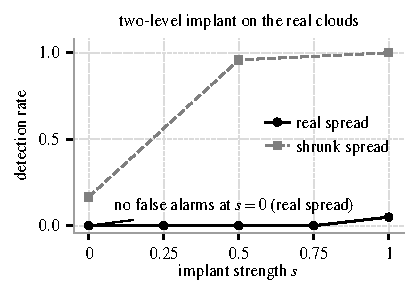
\includegraphics[width=0.5\linewidth]{figures/fig_implant_final.pdf}
\caption{\textbf{A two-level implant on the real ImageNet clouds is missed at the real within-cluster spread and detected once the spread is shrunk.} Detection rate at $z\le-2$ against implant strength $s$ with the real within-cluster spread (solid) and shrunk (dashed): at full strength 0.05 against 1.00, and 0.00 at $s=0$ with the real spread. % expR64b_wn30.csv
}
\label{fig:implant}
\end{figure}
% prov: expR55_depth_power.csv, expR55b_depth_power_leafframe.csv, expR64b_wn30.csv, expR64b_wn30_summary.csv, expR64b_wn30bal_summary.csv, expR67_frame_choice.json, expR69_depth_haarhubs_summary.csv, expR80_implanted_alignment.csv, expR80_decision.csv, expR79_synthetic_deep_poincare.csv, expR81_deep_per_backbone.csv, expR81_deep_per_backbone_summary.csv, expR83_flat_balanced.csv, expR83_flat_balanced_summary.csv
\begin{table}[H]
\centering
\scriptsize
\setlength{\tabcolsep}{2pt}
\begingroup
\footnotesize
\setlength{\tabcolsep}{4pt}
\begin{tabular}{lccccc}
\toprule
cloud & seed & $d$ & excess ($r$) & depth $z$ & decoupled $z$ (cert.) \\
\midrule
three-level hierarchy, ViT-L spectrum & 0 & 1024 & $-0.0081$ (199) & $-1.80$ & $-4.82$ $\pm$ 0.73 (1.0) \\
three-level hierarchy, ViT-L spectrum & 1 & 1024 & $-0.0095$ (199) & $-2.45$ & $-4.44$ $\pm$ 0.58 (1.0) \\
three-level hierarchy, ViT-L spectrum & 2 & 1024 & $-0.0090$ (199) & $-2.38$ & $-4.19$ $\pm$ 0.60 (1.0) \\
three-level hierarchy, ViT-L spectrum & 3 & 1024 & $-0.0099$ (199) & $-2.08$ & $-4.48$ $\pm$ 0.67 (1.0) \\
three-level hierarchy, ViT-L spectrum & 4 & 1024 & $-0.0090$ (199) & $-2.20$ & $-4.28$ $\pm$ 0.54 (1.0) \\
\midrule
flat control, ViT-L spectrum & 0 & 1024 & $-0.0198$ (200) & $-0.08$ & $-1.61$ $\pm$ 0.27 (0.1) \\
flat control, ViT-L spectrum & 1 & 1024 & $-0.0202$ (200) & $-0.32$ & $-1.61$ $\pm$ 0.31 (0.1) \\
flat control, ViT-L spectrum & 2 & 1024 & $-0.0196$ (200) & $-0.20$ & $-1.76$ $\pm$ 0.37 (0.2) \\
flat control, ViT-L spectrum & 3 & 1024 & $-0.0197$ (200) & $-0.69$ & $-1.74$ $\pm$ 0.33 (0.2) \\
flat control, ViT-L spectrum & 4 & 1024 & $-0.0192$ (200) & $-0.27$ & $-1.68$ $\pm$ 0.39 (0.2) \\
\midrule
WordNet Poincar\'e, $d{=}10$ & 0 & 10 & $+0.0830$ (0) & $+2.36$ & $+0.32$ $\pm$ 0.58 (0.0) \\
WordNet Poincar\'e, $d{=}50$ & 0 & 50 & $+0.0354$ (0) & $+1.53$ & $-2.22$ $\pm$ 0.65 (0.6) \\
\bottomrule
\end{tabular}
\par\vspace{2pt}
\endgroup
\caption{\textbf{A deep hierarchy at the real noise level is detected, and a flat control is not.} Synthetic clouds with ViT-L's spectrum and ratio: the depth $z$ intact and decoupled for the hierarchy and for the flat control.
}
\label{tab:q5-power}\label{tab:q5-power-d}
\end{table}


\FloatBarrier
\subsection{Is the island real? The tree map under six configurations}
\label{app:treemap}
Threshold sensitivity of the selection criterion of \S\ref{sec:content}: the selected configuration is stable for degeneracy bounds in $[0.45,0.50]$ on ImageNet and $[0.40,0.50]$ on CIFAR-100; tighter bounds select cosine-complete on ImageNet (gap 0.13) and cosine-Ward on CIFAR-100 (gap 0.56), and in every case the label-free gap is moderate and configuration-sensitive, never a categorical island. The criterion must be applied per dataset: the configuration it selects on DBpedia (Euclidean, average linkage, where nothing is degenerate) is exactly the degenerate naive configuration on ImageNet, so a criterion transferred across datasets would reintroduce the island. % exp23_config_diagnostics.json, exp23_treemap_controls.npz, exp27_dbpedia_treemap.json
\begin{figure}[H]
\centering

\includegraphics[width=0.62\linewidth]{figures/fig_treemap_matrices_final.pdf}
\caption{\textbf{The island is an artifact of the naive cut.} Pairwise ARI between dendrogram cuts under (a) the naive configuration, Euclidean distances with average linkage, where the DINOv2 block agrees with the rest at 0.03, and (b) the selected one, cosine with average linkage, where it agrees at 0.38. % exp23_treemap_controls.npz
}
\label{fig:treemapmat}
\end{figure}
% prov: exp22_tree_similarity_imagenet.npz, exp23_treemap_controls.npz, exp23_config_diagnostics.json, expR58_treemap_cutfree_summary.csv, expR84_tree_ceiling.csv, expR84_tree_ceiling_summary.csv
\begin{table}[H]
\centering
\scriptsize
\setlength{\tabcolsep}{3pt}
\begingroup
\setlength{\tabcolsep}{3pt}
\begin{tabular}{ll|ccc}
\toprule
dataset & configuration & ARI at the cut & cophenetic corr. & triplet agreement \\
\midrule
ImageNet & euclid-average (deg.) & 0.03 / 0.64 & 0.36 / 0.80 & 0.47 / 0.74 \\
ImageNet & euclid-complete (deg.) & 0.03 / 0.44 & 0.20 / 0.66 & 0.41 / 0.65 \\
ImageNet & euclid-ward & 0.16 / 0.53 & 0.62 / 0.84 & 0.67 / 0.85 \\
ImageNet & cosine-average (selected) & 0.39 / 0.48 & 0.48 / 0.78 & 0.77 / 0.76 \\
ImageNet & cosine-complete & 0.13 / 0.49 & 0.18 / 0.72 & 0.36 / 0.71 \\
ImageNet & cosine-ward & 0.17 / 0.55 & 0.59 / 0.85 & 0.69 / 0.86 \\
\midrule
CIFAR-100 & euclid-average (deg.) & 0.00 / 0.57 & 0.15 / 0.78 & 0.41 / 0.74 \\
CIFAR-100 & euclid-complete (deg.) & 0.17 / 0.54 & 0.23 / 0.72 & 0.41 / 0.66 \\
CIFAR-100 & euclid-ward & 0.37 / 0.63 & 0.63 / 0.77 & 0.70 / 0.79 \\
CIFAR-100 & cosine-average (deg.) & 0.30 / 0.58 & 0.42 / 0.72 & 0.51 / 0.64 \\
CIFAR-100 & cosine-complete (selected) & 0.39 / 0.63 & 0.46 / 0.64 & 0.50 / 0.61 \\
CIFAR-100 & cosine-ward & 0.56 / 0.61 & 0.74 / 0.73 & 0.76 / 0.76 \\
\bottomrule
\end{tabular}
\par\vspace{2pt}
\endgroup
\caption{\textbf{The self-supervised models sit apart on distances, not on topology.} The three agreement measures for DINOv2 against the supervised and contrastive models, each written as against those models over within them.
}
\label{tab:q6-treemap}\label{tab:q6-treemap-b}
\end{table}


\FloatBarrier
\subsection{Whose taxonomy? WordNet alignment, superclass recovery, DBpedia and HierarCaps}
\label{app:wordnet}
\label{app:hierarcaps}
On HierarCaps \citep{alper2024hierarcaps} (1000 four-level caption chains), text encoders show the same reading with no class set: the projection radius orders levels within a chain, sibling triplets are resolved at 0.83--0.97 (chance $0.5$), and the leaf excess repeats the text census (Table~\ref{tab:q7-wordnet}). % exp16_hierarcaps.csv
% prov: exp3_alignment.csv, exp28_recovery_per_config.csv, exp8_p1_recovery.csv, exp1_delta_controls.csv, exp8_p6_pooling.csv, expR70_inet1k_supervised.csv, exp14_dbpedia.csv, expR61_dbpedia_record.csv, exp27_dbpedia_treemap.json, exp16_hierarcaps.csv
\begin{table}[H]
\centering
\scriptsize
\setlength{\tabcolsep}{2.6pt}
\begingroup
\footnotesize
\setlength{\tabcolsep}{4pt}
\begin{tabular}{lcccc|c}
\toprule
 & \multicolumn{4}{c|}{Spearman $\rho$, inter-centroid vs WordNet distance} & raw $\hat\delta$ of \\
model & $\rho_{\text{WN}}$ & shuffle & Gaussian & single image & WordNet / random groups \\
\midrule
ViT-T & $+0.52$ & $+0.02$ & $+0.01$ & -- & 0.146 / 0.159 \\
ViT-S & $+0.50$ & $+0.00$ & $-0.00$ & -- & 0.110 / 0.130 \\
ViT-B & $+0.49$ & $+0.03$ & $+0.01$ & -- & 0.092 / 0.120 \\
ViT-L & $+0.53$ & $+0.01$ & $+0.03$ & $+0.25$ & 0.104 / 0.117 \\
\midrule
DINO-B & $+0.36$ & $-0.01$ & $-0.01$ & -- & 0.084 / 0.117 \\
DINOv2-S & $+0.22$ & $+0.01$ & $+0.01$ & -- & 0.077 / 0.100 \\
DINOv2-B & $+0.18$ & $-0.01$ & $+0.01$ & -- & 0.068 / 0.069 \\
DINOv2-L & $+0.18$ & $-0.00$ & $-0.03$ & $+0.08$ & 0.060 / 0.058 \\
DINOv2-G & $+0.20$ & $-0.03$ & $-0.01$ & $+0.03$ & 0.054 / 0.056 \\
\midrule
CLIP-B & $+0.57$ & $+0.00$ & $+0.01$ & -- & 0.126 / 0.174 \\
CLIP-L & $+0.59$ & $+0.01$ & $+0.03$ & $+0.26$ & 0.117 / 0.162 \\
SigLIP-B & $+0.58$ & $-0.01$ & $+0.01$ & -- & 0.118 / 0.158 \\
\midrule
DeiT-B (IN-1k) & $+0.08$ & $+0.01$ & -- & -- & -- \\
ViT-B (augreg, IN-1k) & $+0.52$ & $+0.01$ & -- & -- & -- \\
\bottomrule
\end{tabular}
\par\vspace{2pt}
\endgroup
\caption{\textbf{Agreement with the human taxonomy follows supervision and recipe.} Per backbone on ImageNet: the correlation between inter-centroid and WordNet distances, the same under shuffled labels, a Gaussian cloud and single images, and the raw reading of WordNet against random groups.
}
\label{tab:q7-wordnet}
\end{table}
\begin{table}[H]
\centering
\scriptsize
\setlength{\tabcolsep}{2.6pt}
\begingroup
\setlength{\tabcolsep}{2.5pt}
\begin{tabular}{lcc|cccc|ccc}
\toprule
 & \multicolumn{2}{c|}{supremum, Haar} & \multicolumn{4}{c|}{census} & & & \\
model & $\hat\delta_{\max}$ & excess & $\hat\delta_{99.9}$ & excess & $r$/200 & $p$ & trip.\ & NC H$-$R & FS H$-$R \\
\midrule
BGE-base & 0.122 & -0.032 & 0.082 & -0.021 & 200 & 0.005 & 0.89 & -0.59 & +0.05$\pm$0.05 \\
E5-base & 0.127 & -0.028 & 0.086 & -0.017 & 200 & 0.005 & 0.89 & -0.43 & +0.04$\pm$0.03 \\
GTE-base & 0.132 & -0.024 & 0.088 & -0.017 & 200 & 0.005 & 0.89 & -0.82 & +0.08$\pm$0.06 \\
\bottomrule
\end{tabular}
\par\vspace{2pt}
\endgroup
\caption{\textbf{The recovery is not WordNet circularity.} On DBpedia Classes, an ontology built independently: the reading, the excess, the triplet agreement and the metric gains per text embedder. $r$/200: replicates above the real value.
}
\label{tab:q7-wordnet-c}
\end{table}
\begin{table}[H]
\centering
\scriptsize
\setlength{\tabcolsep}{2.6pt}
\begingroup
\footnotesize
\setlength{\tabcolsep}{4pt}
\begin{tabular}{lcccccc}
\toprule
model & $\rho$(level, radius) & \% monotone & trip.\ L1 & trip.\ L2 & $\hat\delta$ leaves & excess \\
\midrule
BGE-base & +0.80$\pm$0.31 & 49.6 & 0.88 & 0.97 & 0.130 & +0.003 \\
E5-base & +0.87$\pm$0.19 & 53.9 & 0.90 & 0.97 & 0.139 & +0.010 \\
GTE-base & +0.47$\pm$0.55 & 24.0 & 0.90 & 0.97 & 0.135 & +0.006 \\
CLIP-B & +0.64$\pm$0.43 & 27.2 & 0.86 & 0.95 & 0.123 & -0.011 \\
CLIP-L & +0.51$\pm$0.49 & 18.7 & 0.86 & 0.96 & 0.117 & -0.010 \\
SigLIP-B & +0.32$\pm$0.55 & 9.8 & 0.83 & 0.91 & 0.138 & +0.014 \\
\bottomrule
\end{tabular}
\par\vspace{2pt}
\endgroup
\caption{\textbf{A caption hierarchy with no class set reads the same way.} On HierarCaps: the correlation between level and radius, the share of monotone chains, the triplet agreements and the leaf excess per encoder.
}
\label{tab:q7-wordnet-d}
\end{table}


\FloatBarrier
\subsection{Is local structure shared? Permutation-calibrated agreement}
\label{app:local}
% prov: exp21b_local_global_K200.csv
\begin{table}[H]
\centering
\footnotesize
\setlength{\tabcolsep}{3pt}
\begin{tabular}{lcccccc}
\toprule
measure & raw & null mean & $\tau_{0.05}$ & calibrated & null-centered & pairs $p<0.05$ \\
\midrule
mutual-kNN ($k{=}10$), Euclidean & $0.472$ & $0.010$ & $0.015$ & $0.464$ & $0.462$ & 66/66 \\
mutual-kNN, Poincar\'e & $0.425$ & $0.010$ & $0.019$ & $0.414$ & $0.415$ & 66/66 \\
linear CKA, Euclidean & $0.633$ & $0.108$ & $0.111$ & $0.577$ & $0.524$ & 66/66 \\
linear CKA, Poincar\'e & $0.640$ & $0.108$ & $0.111$ & $0.586$ & $0.532$ & 66/66 \\
\bottomrule
\end{tabular}
\par\vspace{2pt}
\caption{\textbf{Cross-model agreement survives permutation calibration.} Columns: the raw measure, the null mean, the calibration threshold, the calibrated value and the number of model pairs that survive, for mutual-kNN agreement and for centroid CKA.
}
\label{tab:q13-local}
\end{table}


\FloatBarrier
\subsection{What follows for practice? The corollary}
\label{app:corollary}
\label{app:familycorr}
\paragraph{One parameter-free projection and two tasks serve the corollary.} The parameter-free map $\phi(x)=\tanh(\tfrac12\|s(x-\mu)\|)\cdot\frac{s(x-\mu)}{\|s(x-\mu)\|}$ centers features, scales the 95th-percentile norm to radius $1/\sqrt2$, and preserves directions; prototypes in the ball are means of projected points re-mapped through the origin. Tasks: nearest-centroid (NC) and 5-way 5-shot (FS, 1000 paired episodes); metric arms: Euclidean (R), Poincar\'{e} (H), the radial map with Euclidean distances (RT), cosine (COS), and the L2-normalized stack. Changing the readout metric on the intact configuration, which is what the rule selects among, is distinct from deforming the configuration itself. % exp1, exp2

\paragraph{Both readings predict the gain within datasets.} Within each hierarchical dataset the Poincar\'{e} advantage tracks the record excess: the nearest-centroid correlation is $-0.73$ on ImageNet with a confidence interval that excludes zero on all four datasets, the few-shot correlation excludes zero on CIFAR-100, CIFAR-10 and DTD but not on ImageNet, and the hierarchy-test $z$ predicts no gain anywhere (Table~\ref{tab:q9-corollary}). The raw reading correlates as strongly ($-0.84$ on ImageNet for nearest-centroid) and survives partialing out dimension, baseline accuracy, family and spectral covariates; without DINOv2 it holds on ImageNet and CIFAR-100 but not on CIFAR-10/DTD. Pooled cross-dataset correlations are family-driven and not used as evidence; on flat-label datasets no metric helps. Gains carry paired confidence intervals and a McNemar test. % expR68_corollary_excess.csv, table1_regenerated.csv, night/correlation_cis.csv, exp13_mcnemar.csv

\paragraph{The training objective picks the metric.} The radial map with Euclidean distances changes nothing, so the gain is the metric itself, and the split follows the objective: cosine suffices for DINOv2, Poincar\'{e} $\approx$ cosine for supervised ViTs, and Poincar\'{e} beats cosine for CLIP by up to +1.3pp even after L2 normalization (Table~\ref{tab:q9-corollary}). The rule is read off the families it is scored on: it describes them rather than validating a policy. % exp2, exp2b, exp24

\paragraph{A diagnostic, not a policy.} \citet{Khrulkov_2020_CVPR} estimate $c\approx0.33$ from the raw reading of their datasets; the same rule on structureless Gaussian clouds gives the curvatures of Section~\ref{sec:practice}. Cosine is a safe default, gating on the reading is the weakest policy tested, and gains are modest and limited to prototype-based tasks (sample-level tasks never benefit, Table~\ref{tab:q3-sample}). On DBpedia, a three-level text hierarchy, the diagnostic predicts correctly on both sides: genuine excess, no metric gain. % exp2, exp20, exp24, exp14, exp15
% prov: table1_regenerated.csv, exp2_metric_controls.csv, exp2b_normalized_stack.csv, exp13_mcnemar.csv, night/correlation_cis.csv, exp20_null_ztable.csv, expR68_corollary_excess.csv, exp24_val_metric_selection.csv, night/t_sweep.csv
\begin{table}[tbp]
\centering
\scriptsize
\setlength{\tabcolsep}{2.6pt}
\begingroup
\noindent\textbf{(a) Task accuracies and zero-cost metric gains per cell (10 backbones with cached per-dataset features $\times$ 6 datasets).}\par\vspace{1.5pt}
\scriptsize\renewcommand{\arraystretch}{0.88}
\setlength{\tabcolsep}{3pt}
\begin{tabular}{llcccccccc}
\toprule
 & & \multicolumn{2}{c}{NC acc.\ (\%)} & \multicolumn{2}{c}{FS acc.\ (\%)} & \multicolumn{3}{c}{FS advantage over Euclidean (pp)} & McNemar \\
\cmidrule(lr){3-4}\cmidrule(lr){5-6}\cmidrule(lr){7-9}
model & data & Eucl. & Poinc. & Eucl. & Poinc. & cosine & radial map & Poinc.$_{\text{N}}$ $-$ cos & NC H vs R \\
\midrule
ViT-T & IN & 68.1 & 67.2 & 97.5 & 97.6 & -0.01 & +0.01 & +0.08 & $10^{-22}$\,($-$) \\
 & C100 & 29.3 & 28.2 & 62.4 & 63.1 & +1.01 & +0.45 & +0.55 & $10^{-5}$\,($-$) \\
 & C10 & 87.5 & 87.4 & 87.6 & 88.1 & +0.66 & +0.19 & +0.29 & 0.19\,($-$) \\
 & DTD & 63.7 & 62.5 & 83.3 & 83.9 & -0.23 & +0.32 & +0.69 & 0.03\,($-$) \\
 & FMNIST & 78.5 & 78.4 & 81.6 & 81.9 & +0.21 & +0.10 & +0.31 & 0.38\,($-$) \\
 & MNIST & 75.9 & 74.0 & 74.3 & 74.6 & +0.64 & +0.52 & +0.20 & $10^{-13}$\,($-$) \\
\midrule
ViT-S & IN & 77.7 & 77.5 & 98.6 & 98.7 & +0.17 & -0.02 & -0.07 & 0.09\,($-$) \\
 & C100 & 74.9 & 74.6 & 92.2 & 92.4 & +0.59 & +0.16 & -0.00 & 0.10\,($-$) \\
 & C10 & 93.4 & 93.2 & 92.0 & 92.5 & +0.56 & +0.27 & +0.19 & 0.02\,($-$) \\
 & DTD & 69.3 & 68.5 & 85.4 & 86.0 & -0.03 & +0.25 & +0.73 & 0.10\,($-$) \\
 & FMNIST & 80.7 & 80.4 & 83.7 & 83.5 & +0.28 & +0.08 & -0.19 & 0.08\,($-$) \\
 & MNIST & 84.8 & 84.1 & 80.5 & 81.4 & +0.34 & +0.65 & +0.84 & $10^{-4}$\,($-$) \\
\midrule
ViT-B & IN & 81.6 & 81.7 & 98.9 & 99.0 & +0.20 & -0.04 & -0.05 & 0.21\,(+) \\
 & C100 & 77.3 & 77.0 & 92.5 & 92.7 & +0.56 & +0.12 & -0.05 & 0.07\,($-$) \\
 & C10 & 94.5 & 94.0 & 92.7 & 93.0 & +0.49 & +0.18 & +0.15 & $10^{-5}$\,($-$) \\
 & DTD & 70.8 & 70.8 & 85.4 & 86.2 & +0.28 & +0.19 & +0.69 & 1.00\,($-$) \\
 & FMNIST & 81.3 & 81.6 & 83.4 & 83.3 & +0.03 & +0.09 & -0.04 & 0.08\,(+) \\
 & MNIST & 81.6 & 80.5 & 76.8 & 77.6 & +0.19 & +0.51 & +0.66 & $10^{-7}$\,($-$) \\
\midrule
ViT-L & IN & 86.1 & 86.2 & 99.4 & 99.4 & +0.11 & -0.03 & -0.02 & 0.58\,(+) \\
 & C100 & 85.3 & 85.2 & 94.8 & 95.5 & +1.17 & +0.31 & +0.12 & 0.59\,($-$) \\
 & C10 & 97.5 & 97.5 & 95.0 & 95.8 & +1.25 & +0.35 & +0.59 & 0.76\,(+) \\
 & DTD & 71.8 & 71.5 & 85.6 & 86.5 & +0.13 & +0.16 & +1.02 & 0.69\,($-$) \\
 & FMNIST & 83.7 & 83.5 & 84.4 & 84.7 & +0.00 & +0.17 & +0.23 & 0.12\,($-$) \\
 & MNIST & 84.2 & 83.6 & 80.8 & 81.6 & +0.08 & +0.42 & +0.67 & 0.00\,($-$) \\
\midrule
DINOv2-S & IN & 74.7 & 74.4 & 97.4 & 97.9 & +0.68 & +0.03 & -0.22 & 0.00\,($-$) \\
 & C100 & 73.4 & 74.4 & 94.3 & 95.1 & +0.80 & +0.15 & +0.06 & $10^{-6}$\,(+) \\
 & C10 & 95.0 & 95.2 & 92.9 & 93.5 & -0.36 & +0.13 & +1.06 & 0.14\,(+) \\
 & DTD & 73.4 & 73.4 & 89.8 & 90.5 & +0.30 & +0.04 & +0.36 & 1.00\,(+) \\
 & FMNIST & 82.2 & 82.2 & 85.4 & 85.5 & +0.02 & +0.07 & +0.07 & 1.00\,($-$) \\
 & MNIST & 83.4 & 81.9 & 80.2 & 80.8 & -0.07 & +0.45 & +0.67 & $10^{-11}$\,($-$) \\
\midrule
DINOv2-B & IN & 78.9 & 78.9 & 97.0 & 97.8 & +1.40 & +0.04 & -0.63 & 0.57\,(+) \\
 & C100 & 87.4 & 87.9 & 96.5 & 97.2 & +1.11 & +0.09 & -0.34 & $10^{-4}$\,(+) \\
 & C10 & 97.1 & 97.4 & 94.7 & 95.4 & +0.27 & +0.03 & +0.43 & $10^{-4}$\,(+) \\
 & DTD & 74.2 & 74.7 & 89.2 & 90.3 & +1.48 & +0.01 & -0.35 & 0.31\,(+) \\
 & FMNIST & 83.2 & 82.8 & 85.9 & 85.9 & +0.21 & +0.04 & -0.18 & 0.01\,($-$) \\
 & MNIST & 80.6 & 78.8 & 76.6 & 77.1 & +0.17 & +0.48 & +0.47 & $10^{-16}$\,($-$) \\
\midrule
DINOv2-L & IN & 79.8 & 80.4 & 96.2 & 97.1 & +2.13 & +0.02 & -1.24 & $10^{-14}$\,(+) \\
 & C100 & 85.6 & 87.7 & 96.1 & 97.1 & +1.80 & +0.09 & -0.74 & $10^{-38}$\,(+) \\
 & C10 & 97.9 & 98.3 & 94.1 & 95.1 & +0.92 & -0.00 & +0.11 & $10^{-8}$\,(+) \\
 & DTD & 74.4 & 75.2 & 87.1 & 88.4 & +2.40 & +0.03 & -0.98 & 0.11\,(+) \\
 & FMNIST & 84.4 & 84.5 & 87.8 & 87.9 & +0.29 & +0.03 & -0.03 & 0.40\,(+) \\
 & MNIST & 74.1 & 72.7 & 70.5 & 71.1 & +0.25 & +0.43 & +0.46 & $10^{-12}$\,($-$) \\
\midrule
DINOv2-G & IN & 78.4 & 78.3 & 96.2 & 97.1 & +2.57 & +0.03 & -1.65 & 0.10\,($-$) \\
 & C100 & 89.8 & 91.0 & 95.9 & 97.2 & +2.44 & +0.13 & -1.10 & $10^{-16}$\,(+) \\
 & C10 & 97.8 & 98.2 & 92.3 & 93.8 & +2.51 & -0.02 & -1.01 & $10^{-13}$\,(+) \\
 & DTD & 72.9 & 73.1 & 87.2 & 88.5 & +2.63 & +0.01 & -1.38 & 0.81\,(+) \\
 & FMNIST & 85.9 & 85.8 & 89.0 & 89.2 & +0.38 & +0.04 & -0.07 & 0.72\,($-$) \\
 & MNIST & 79.3 & 78.6 & 72.9 & 73.8 & +0.30 & +0.56 & +0.72 & 0.00\,($-$) \\
\midrule
CLIP-B & IN & 61.4 & 59.9 & 96.8 & 96.8 & -0.04 & -0.00 & +0.14 & $10^{-40}$\,($-$) \\
 & C100 & 65.6 & 65.1 & 87.7 & 88.9 & -0.03 & +0.44 & +1.21 & 0.07\,($-$) \\
 & C10 & 87.9 & 88.3 & 89.5 & 90.1 & -0.19 & +0.20 & +0.90 & $10^{-4}$\,(+) \\
 & DTD & 63.7 & 63.2 & 82.2 & 83.1 & -0.23 & +0.36 & +1.29 & 0.46\,($-$) \\
 & FMNIST & 75.9 & 75.1 & 78.8 & 78.9 & +0.06 & +0.17 & +0.10 & $10^{-4}$\,($-$) \\
 & MNIST & 70.1 & 66.6 & 70.9 & 69.7 & +0.04 & +0.23 & -1.17 & $10^{-45}$\,($-$) \\
\midrule
CLIP-L & IN & 75.0 & 74.5 & 98.4 & 98.6 & +0.01 & +0.00 & +0.22 & $10^{-8}$\,($-$) \\
 & C100 & 74.6 & 74.5 & 90.0 & 90.8 & +0.12 & +0.39 & +1.23 & 0.66\,($-$) \\
 & C10 & 95.9 & 95.9 & 92.4 & 93.0 & +0.16 & +0.25 & +0.91 & 0.59\,($-$) \\
 & DTD & 68.6 & 69.0 & 85.2 & 86.2 & -0.08 & +0.36 & +1.24 & 0.45\,(+) \\
 & FMNIST & 76.2 & 75.9 & 76.8 & 77.3 & +0.12 & +0.33 & +0.68 & 0.09\,($-$) \\
 & MNIST & 85.2 & 86.1 & 83.7 & 84.7 & +0.08 & +0.58 & +1.06 & $10^{-7}$\,(+) \\
\bottomrule
\end{tabular}
\par\vspace{5pt}
\endgroup
\caption{\textbf{Both readings predict the zero-cost gain within datasets, the depth verdict predicts nothing, and cosine is the safe default.} (a) Nearest-centroid (NC) and 5-way 5-shot (FS, 1000 paired episodes) accuracy under Euclidean and Poincar\'e readouts, regenerated from the audited reruns; FS advantage of cosine and of the radial map with Euclidean distances (the map without the metric changes nothing) over Euclidean, and of the Poincar\'e readout over cosine after L2 normalization; McNemar $p$ for the NC test-set decisions, Poincar\'e vs Euclidean (order of magnitude when $p<10^{-3}$; sign of the NC advantage in parentheses). % table1_regenerated.csv, exp2_metric_controls.csv, exp2b_normalized_stack.csv, exp13_mcnemar.csv
}
\label{tab:q9-corollary}
\end{table}
\begin{table}[tbp]\ContinuedFloat
\centering
\scriptsize
\setlength{\tabcolsep}{2.6pt}
\begingroup
\noindent\textbf{(c) Best zero-cost metric per backbone: few-shot advantage over Euclidean, mean over the four hierarchical datasets, and which metric collects it (either: within $0.15$pp).}\par\vspace{1.5pt}
\footnotesize
\setlength{\tabcolsep}{5pt}
\begin{tabular}{lcc}
\toprule
model & best$-$R (pp) & metric \\
\midrule
ViT-T & $+0.58$ & either \\
ViT-S & $+0.49$ & either \\
ViT-B & $+0.51$ & either \\
ViT-L & $+0.87$ & either \\
DINOv2-S & $+0.68$ & H \\
DINOv2-B & $+1.17$ & cos \\
DINOv2-L & $+1.84$ & cos \\
DINOv2-G & $+2.54$ & cos \\
CLIP-B & $+0.67$ & H \\
CLIP-L & $+0.65$ & H \\
\bottomrule
\end{tabular}
\par\vspace{5pt}
\endgroup
\caption{(continued)}
\end{table}
\begin{table}[tbp]\ContinuedFloat
\centering
\scriptsize
\setlength{\tabcolsep}{2.6pt}
\begingroup
\noindent\textbf{(d) The same correlations on the raw $\hat\delta_{99.9}$, the record excess and the depth-test $z$ (Fisher-$z$ CI95; dm: family-demeaned $r$).}\par\vspace{1.5pt}
\setlength{\tabcolsep}{3pt}
\begin{tabular}{llcc|cc|c}
\toprule
 & & \multicolumn{2}{c|}{raw $\hat\delta_{99.9}$} & \multicolumn{2}{c|}{record excess} & depth $z$ \\
gain & dataset & $r$ [CI95] & dm & $r$ [CI95] & dm & $r$ [CI95] \\
\midrule
NC H$-$R & ImageNet & $-0.84$ [-0.96, -0.45] & $-0.83$ & $-0.73$ [-0.93, -0.19] & $-0.61$ & $-0.28$ [-0.77, +0.42] \\
 & CIFAR-100 & $-0.92$ [-0.98, -0.68] & $-0.58$ & $-0.79$ [-0.95, -0.33] & $-0.21$ & $+0.52$ [-0.16, +0.87] \\
 & CIFAR-10 & $-0.63$ [-0.90, +0.00] & $-0.31$ & $-0.67$ [-0.91, -0.06] & $-0.34$ & n/a \\
 & DTD & $-0.67$ [-0.91, -0.07] & $-0.67$ & $-0.76$ [-0.94, -0.26] & $-0.60$ & n/a \\
\midrule
FS H$-$R & ImageNet & $-0.86$ [-0.97, -0.50] & $-0.56$ & $-0.21$ [-0.74, +0.48] & $+0.35$ & $+0.27$ [-0.43, +0.77] \\
 & CIFAR-100 & $-0.62$ [-0.90, +0.02] & $-0.51$ & $-0.79$ [-0.95, -0.31] & $-0.80$ & $-0.26$ [-0.76, +0.45] \\
 & CIFAR-10 & $-0.78$ [-0.95, -0.31] & $-0.64$ & $-0.78$ [-0.95, -0.30] & $-0.66$ & n/a \\
 & DTD & $-0.87$ [-0.97, -0.53] & $-0.94$ & $-0.98$ [-1.00, -0.91] & $-0.97$ & n/a \\
\midrule
FS best$-$R & ImageNet & $-0.83$ [-0.96, -0.43] & $-0.50$ & $-0.08$ [-0.68, +0.58] & $+0.47$ & $+0.13$ [-0.54, +0.70] \\
 & CIFAR-100 & $-0.77$ [-0.94, -0.27] & $-0.75$ & $-0.75$ [-0.94, -0.23] & $-0.65$ & $+0.22$ [-0.48, +0.75] \\
 & CIFAR-10 & $-0.63$ [-0.90, -0.01] & $-0.55$ & $-0.62$ [-0.90, +0.02] & $-0.56$ & n/a \\
 & DTD & $-0.81$ [-0.95, -0.36] & $-0.78$ & $-0.90$ [-0.98, -0.63] & $-0.84$ & n/a \\
\bottomrule
\end{tabular}
\par\vspace{5pt}
\endgroup
\caption{(continued) (d) The calibrated reading: the raw 99.9th-percentile statistic, the record excess and the depth-test $z$ of Table~\ref{tab:q4-depth} as predictors. (e) Validation picking retains the oracle advantage and the zero-validation objective rule modestly beats always-cosine. (f) The gate's value is avoiding the Poincar\'e projection on flat-label data; cosine is a safe NC default everywhere. (g) The headline $t=1/\sqrt2\approx0.71$ was fixed a priori and is conservative for FS. % expR68_corollary_excess.csv, exp24_val_metric_selection.csv, night/t_sweep.csv
}
\end{table}
\begin{table}[tbp]\ContinuedFloat
\centering
\scriptsize
\setlength{\tabcolsep}{2.6pt}
\begingroup
\noindent\textbf{(e) Few-shot metric-selection policies on held-out episodes (500 validation / 500 test per cell).}\par\vspace{1.5pt}
\footnotesize
\setlength{\tabcolsep}{5pt}
\begin{tabular}{lcc}
\toprule
policy (test advantage over Euclidean, pp) & all 60 cells & hierarchical (40) \\
\midrule
always cosine & +0.23 & +0.28 \\
objective rule (zero validation) & +0.28 & +0.41 \\
$\delta$-gated objective rule & +0.08 & +0.13 \\
validation-picked per cell & +0.63 & +0.78 \\
test oracle (reference) & +0.64 & +0.78 \\
\bottomrule
\end{tabular}
\par\vspace{5pt}
\endgroup
\caption{(continued)}
\end{table}
\begin{table}[tbp]\ContinuedFloat
\centering
\scriptsize
\setlength{\tabcolsep}{2.6pt}
\begingroup
\noindent\textbf{(f) Nearest-centroid metric-selection policies.}\par\vspace{1.5pt}
\footnotesize
\setlength{\tabcolsep}{5pt}
\begin{tabular}{lccc}
\toprule
NC policy (advantage over Euclidean, pp) & all 60 & flat (20) & hierarchical (40) \\
\midrule
always cosine & +0.48 & +0.24 & +0.59 \\
always Poincar\'e & -0.24 & -0.70 & -0.00 \\
gated rule (flat$\to$R) & +0.34 & +0.00 & +0.51 \\
$\delta$-gated rule & +0.19 & +0.00 & +0.29 \\
\bottomrule
\end{tabular}
\par\vspace{5pt}
\endgroup
\caption{(continued)}
\end{table}
\begin{table}[tbp]\ContinuedFloat
\centering
\scriptsize
\setlength{\tabcolsep}{2.6pt}
\begingroup
\noindent\textbf{(g) Sensitivity to the projection target $t$ (36 hierarchical cells).}\par\vspace{1.5pt}
\footnotesize
\setlength{\tabcolsep}{5pt}
\begin{tabular}{lcccccccc}
\toprule
target $t$ & 0.25 & 0.35 & 0.41 & 0.45 & 0.50 & 0.58 & 0.71 & 0.95 \\
\midrule
FS adv.\ mean (pp) & +0.88 & +0.87 & +0.87 & +0.86 & +0.84 & +0.82 & +0.76 & +0.56 \\
NC adv.\ mean (pp) & -0.30 & -0.25 & -0.23 & -0.21 & -0.17 & -0.12 & -0.01 & +0.15 \\
\% cells FS $>0$ & 97 & 100 & 100 & 100 & 100 & 100 & 100 & 100 \\
\bottomrule
\end{tabular}
\par\vspace{5pt}
\endgroup
\caption{(continued)}
\end{table}


\FloatBarrier
\subsection{Provenance}
\label{app:provenance}
\begin{table}[tbp]
\centering
\scriptsize
\setlength{\tabcolsep}{3pt}
\begin{tabular}{ll>{\raggedright\arraybackslash}p{9.0cm}}
\toprule
table & generated file & result file(s) \\
\midrule
\ref{tab:q1-census} & \texttt{tab\_q01\_census\_final} & \texttt{expR75\_census\_centered\_haar.csv} \texttt{expR52\_census\_haar\_p999\_200.csv} \texttt{expR54\_census\_haar\_sup\_200.csv} \texttt{expR40b\_p999census200.csv} \texttt{expR39c\_census200\_cache.csv} \texttt{expR57\_census\_cosine\_haar\_p999\_200.csv} \texttt{expR57\_text\_cosine\_haar\_p999\_200.csv} \texttt{exp10\_local\_vs\_global.csv} \texttt{expR45\_convnet\_rows.csv} \texttt{exp20\_null\_ztable.csv} \\
\ref{tab:q2-text} & \texttt{tab\_q02\_text} & \texttt{expR53\_text\_haar\_p999\_200.csv} \texttt{expR53\_text\_haar\_sup\_200.csv} \texttt{expR53\_text\_gauss\_p999\_200.csv} \texttt{expR48b\_text\_census200\_bs1.csv} \texttt{expR57\_text\_cosine\_haar\_p999\_200.csv} \texttt{exp18\_text\_nulls.csv} \texttt{exp4\_prompt\_variation.csv} \texttt{exp17\_wordnet\_prompts.csv} \texttt{expR49\_template\_nulls\_bs1.csv} \texttt{expR47\_extraction\_variance.csv} \\
\ref{tab:q3-sample} & \texttt{tab\_q03\_sample\_final} & \texttt{expR62\_samplelevel\_record.csv} \texttt{expR78\_khrulkov\_replication.csv} \texttt{expR78\_khrulkov\_replication\_summary.csv} \\
\ref{tab:q4-depth} & \texttt{tab\_q04\_depth\_final} & \texttt{expR56\_depth\_variants.csv} \texttt{expR69\_depth\_haarhubs\_summary.csv} \texttt{expR64b\_wn30bal\_summary.csv} \texttt{expR70\_inet1k\_supervised.csv} \texttt{expR52\_census\_haar\_p999\_200.csv} \texttt{expR63\_meru\_record.csv} \texttt{expR65\_hier\_finetune.csv} \texttt{expR74\_decoupling\_summary.csv} \texttt{expR71\_meru\_radii.csv} \texttt{expR77\_positive\_control.csv} \texttt{expR77\_positive\_control\_verdict.json} \texttt{expR82\_radial\_control.csv} \texttt{expR82\_radial\_control\_summary.csv} \\
\ref{tab:q5-power} & \texttt{tab\_q05\_power\_final} & \texttt{expR55\_depth\_power.csv} \texttt{expR55b\_depth\_power\_leafframe.csv} \texttt{expR64b\_wn30.csv} \texttt{expR64b\_wn30\_summary.csv} \texttt{expR64b\_wn30bal\_summary.csv} \texttt{expR67\_frame\_choice.json} \texttt{expR69\_depth\_haarhubs\_summary.csv} \texttt{expR80\_implanted\_alignment.csv} \texttt{expR80\_decision.csv} \texttt{expR79\_synthetic\_deep\_poincare.csv} \texttt{expR81\_deep\_per\_backbone.csv} \texttt{expR81\_deep\_per\_backbone\_summary.csv} \texttt{expR83\_flat\_balanced.csv} \texttt{expR83\_flat\_balanced\_summary.csv} \\
\ref{tab:q6-treemap} & \texttt{tab\_q06\_treemap} & \texttt{exp22\_tree\_similarity\_imagenet.npz} \texttt{exp23\_treemap\_controls.npz} \texttt{exp23\_config\_diagnostics.json} \texttt{expR58\_treemap\_cutfree\_summary.csv} \texttt{expR84\_tree\_ceiling.csv} \texttt{expR84\_tree\_ceiling\_summary.csv} \\
\ref{tab:q7-wordnet} & \texttt{tab\_q07\_wordnet\_final} & \texttt{exp3\_alignment.csv} \texttt{exp28\_recovery\_per\_config.csv} \texttt{exp8\_p1\_recovery.csv} \texttt{exp1\_delta\_controls.csv} \texttt{exp8\_p6\_pooling.csv} \texttt{expR70\_inet1k\_supervised.csv} \texttt{exp14\_dbpedia.csv} \texttt{expR61\_dbpedia\_record.csv} \texttt{exp27\_dbpedia\_treemap.json} \texttt{exp16\_hierarcaps.csv} \\
\ref{tab:q8-robust} & \texttt{tab\_q08\_robust\_final} & \texttt{expR72\_budget\_record.csv} \texttt{expR72\_budget\_record\_summary.csv} \texttt{expR59\_imagenet\_bootstrap\_summary.csv} \texttt{expR73\_transfer\_bootstrap\_record\_summary.csv} \texttt{expR66\_joint\_sensitivity\_summary.csv} \texttt{expR60\_c\_sweep\_record.csv} \texttt{analysis4\_finetuning.csv} \texttt{e1\_delta\_by\_layer.csv} \texttt{expR66c\_joint\_sensitivity\_summary.csv} \\
\ref{tab:q9-corollary} & \texttt{tab\_q09\_corollary} & \texttt{table1\_regenerated.csv} \texttt{exp2\_metric\_controls.csv} \texttt{exp2b\_normalized\_stack.csv} \texttt{exp13\_mcnemar.csv} \texttt{night/correlation\_cis.csv} \texttt{exp20\_null\_ztable.csv} \texttt{expR68\_corollary\_excess.csv} \texttt{exp24\_val\_metric\_selection.csv} \texttt{night/t\_sweep.csv} \\
\ref{tab:q10-calibration} & \texttt{tab\_q10\_calibration} & \texttt{exp1\_delta\_controls.csv} \texttt{expR42\_star\_calibration.csv} \\
\ref{tab:q13-local} & \texttt{tab\_q13\_local} & \texttt{exp21b\_local\_global\_K200.csv} \\
\ref{tab:q14-panel} & \texttt{tab\_q14\_panel} & \texttt{(model panel: stated in the generator; parameter counts from the model cards)} \\
\bottomrule
\end{tabular}
\caption{Provenance index: every table of this appendix is generated by script from the result files listed here; no table value is hand-transcribed. The same mapping for the main text is annotated in the source and shipped with the code release.}
\label{tab:provenance}
\end{table}




\end{document}
